\RequirePackage[ngerman=ngerman-x-latest]{hyphsubst}

\documentclass[ngerman, cd=lightcolor]{tudscrreprt}

% Packages
\usepackage{caption}
\usepackage{calc}
\usepackage{babel}
\usepackage{enumitem}
\usepackage{graphicx}
\usepackage{hyperref}
\usepackage[utf8]{inputenc}
\usepackage[outputdir=aux]{minted}
\usepackage{xcolor}

% Import after xcolor to avoid clash
\usepackage{svg}

% Settings
\setcounter{secnumdepth}{3}
\setcounter{tocdepth}{3}
\setlength{\footnotesep}{\baselineskip}
\setminted{%
  frame=single,
  fontsize=\scriptsize,
  labelposition=none,
}
\captionsetup[listing]{position=above,skip=-5pt}

% Hierarchical listing numbering
\makeatletter
\def\counterwithin@x#1#2{%
  \@ifbothcounters{#1}{#2}%
      {\@addtoreset{#1}{#2}%
       \expandafter
       \gdef\csname the#1\expandafter\endcsname\expandafter
            {\csname the#2\expandafter\endcsname\expandafter
             .\expandafter
           %^^^
             \@arabic\csname c@#1\endcsname}}}
\makeatother
\counterwithin{listing}{chapter}

% Overlined text
\makeatletter
\newcommand*{\textoverline}[1]{$\overline{\hbox{#1}}\m@th$}
\makeatother

% Document
\begin{document}

\faculty{Fakultät für Elektrotechnik und Informationstechnik}
\institute{Institut für Grundlagen der Elektrotechnik und Elektronik}
\chair{Professur für hochparallele VLSI-Systeme und Neuromikroelektronik}

\title{Belegarbeit VLSI-Prozessorentwurf}

\author{%
  Adrian Zinke%
  \discipline{ET}%
  \matriculationnumber{3905879}%
\and%
  Timo Nicolai%
  \discipline{IST}%
  \matriculationnumber{4048209}%
\and%
  SVN-Gruppennummer: Gruppe02%
}

\headingsvskip=-100pt

\maketitle
\tableofcontents
\pagebreak

\sloppy

\vspace*{100px}

\centerline{\textbf{Selbstständigkeitserklärung}}

\vspace{10px}

\noindent
Hiermit versichern wir, dass wir die vorliegende Arbeit mit dem Titel
\textit{Belegarbeit VLSI-Prozessorentwurf} selbstständig und ohne unzulässige
Hilfe Dritter verfasst haben. Es wurden keine anderen als die in der Arbeit
angegebenen Hilfsmittel und Quellen benutzt. Es waren keine weiteren Personen
an der geistigen Herstellung der vorliegenden Arbeit beteiligt. Uns ist
bekannt, dass die Nichteinhaltung dieser Erklärung zum nachträglichen Entzug
des Hochschulabschlusses führen kann.

\vspace{10px}

\noindent
Dresden, \today

\vspace{40px}

\noindent
Adrian Zinke

\vspace{40px}

\noindent
Timo Nicolai

\chapter{Einleitung}

Mikroprozessoren sind aus unserer heutigen Gesellschaft nicht mehr wegzudenken.
Man findet sie in Handys, PCs, Autos und Herzschrittmachern, um nur einige
wenige Beispiele zu nennen. Im Modul \textit{VLSI-Prozessorentwurf} bestand die
Aufgabe darin, einen Teil des Entwicklungszyklus eines Mikroprozessors anhand
des Beispiels einer mit Zilog Z80 Bytecode kompatiblen integrierten Schaltung
nachzuvollziehen. Dies beinhaltet deren Entwurf, Implementierung sowie
Verifikation per Simulation und anschließende Synthese und Layout.

In diesem Bericht wird zuerst auf die von uns verfolgten Design-Ziele und
anschließend auf die Struktur unseres Verilog-Codes und die
Implementierungsdetails der wichtigsten Module eingegangen. Anschließend folgt
eine Betrachtung des von unserer Implementierung während Speicher- und IO
Zugriffen gezeigten Timings. Danach wird auf die Verifikation und dabei
insbesondere auf unsere Ansätze zur Automatisierung des Verifikationsprozesses
eingegangen.  Das darauffolgende Kapitel beschreibt die von uns getroffenen
Maßnahmen um unsere Implementierung bezüglich der von uns gesetzten Design
Ziele zu optimieren und den dabei erzielten Erfolg. Anschließend werden die
Ergebnisse der Synthese und Place \& Route Schritte präsentiert. Zuletzt
erfolgt eine kurze Einschätzung und Bewertung der Arbeit.

\chapter{Design-Ziele\label{ch:design-goals}}

Oberste Priorität hat die korrekte Funktionalität unserer Implementierung.
Entsprechend ist ein großer Teil des Entwicklungsaufwandes in die Verifizierung
geflossen.

Als Optimierungsziel haben wir uns auf die Geschwindigkeit des Prozessors
festgelegt. Die erreichte Geschwindigkeit hängt dabei sowohl von der maximalen
Taktfrequenz der resultierenden Schaltung als auch der Länge der einzelnen
Instruktionen in Takten ab. Das exakte Optimierungsziel ist hier ohne
Betrachtung konkreter Benchmark-Programme nicht klar definiert, da das Einfügen
zusätzlicher Takte in einige Instruktionen unter Umständen eine Erhöhung
der Taktfrequenz ermöglicht, wenn hierbei zusätzliche Register auf dem
kritischen Pfad eingefügt werden können. Hier lässt sich also maximal ein
Pareto-Optimum erreichen. Das Anlegen von Benchmark-Programmen ist wiederum
nicht trivial, da nicht bekannt ist, in welchen Bereichen der entwickelte
Prozessor eingesetzt werden soll.  Beispielsweise ist es schwierig zu
entscheiden, ob die Geschwindigkeit der 16-Bit ALU-Operationen genauso wichtig
ist wie die der 8-Bit ALU-Operationen.  Dies kann aber zum Beispiel die
Entscheidung für oder gegen eine 16-Bit ALU beeinflussen.

Wir haben mit dem Ansatz gearbeitet, zunächst alle Instruktionen so zu
implementieren, dass ihre Länge in Takten dem unteren Limit entspricht, das
durch die während der Instruktion notwendigen Speicherzugriffe bestimmt ist.
Anschließend wurde unter Beibehaltung dieser Instruktions-Längen die
Taktfrequenz optimiert. Erst danach wurde versucht, durch Einfügen zusätzlicher
Takte die Taktfrequenz noch weiter zu erhöhen. Ob der dabei erzielte
Taktfrequenz-Gewinn die Verlängerung der betroffenen Instruktionen wert ist
wurde dann von Fall zu Fall nicht formal sondern rein intuitiv entschieden.
Die erzielten Ergebnisse sind in Abschnitt~\ref{ch:syn} dokumentiert.

\chapter{Modulbeschreibungen}

\begin{figure}[htbp]
  \centering
    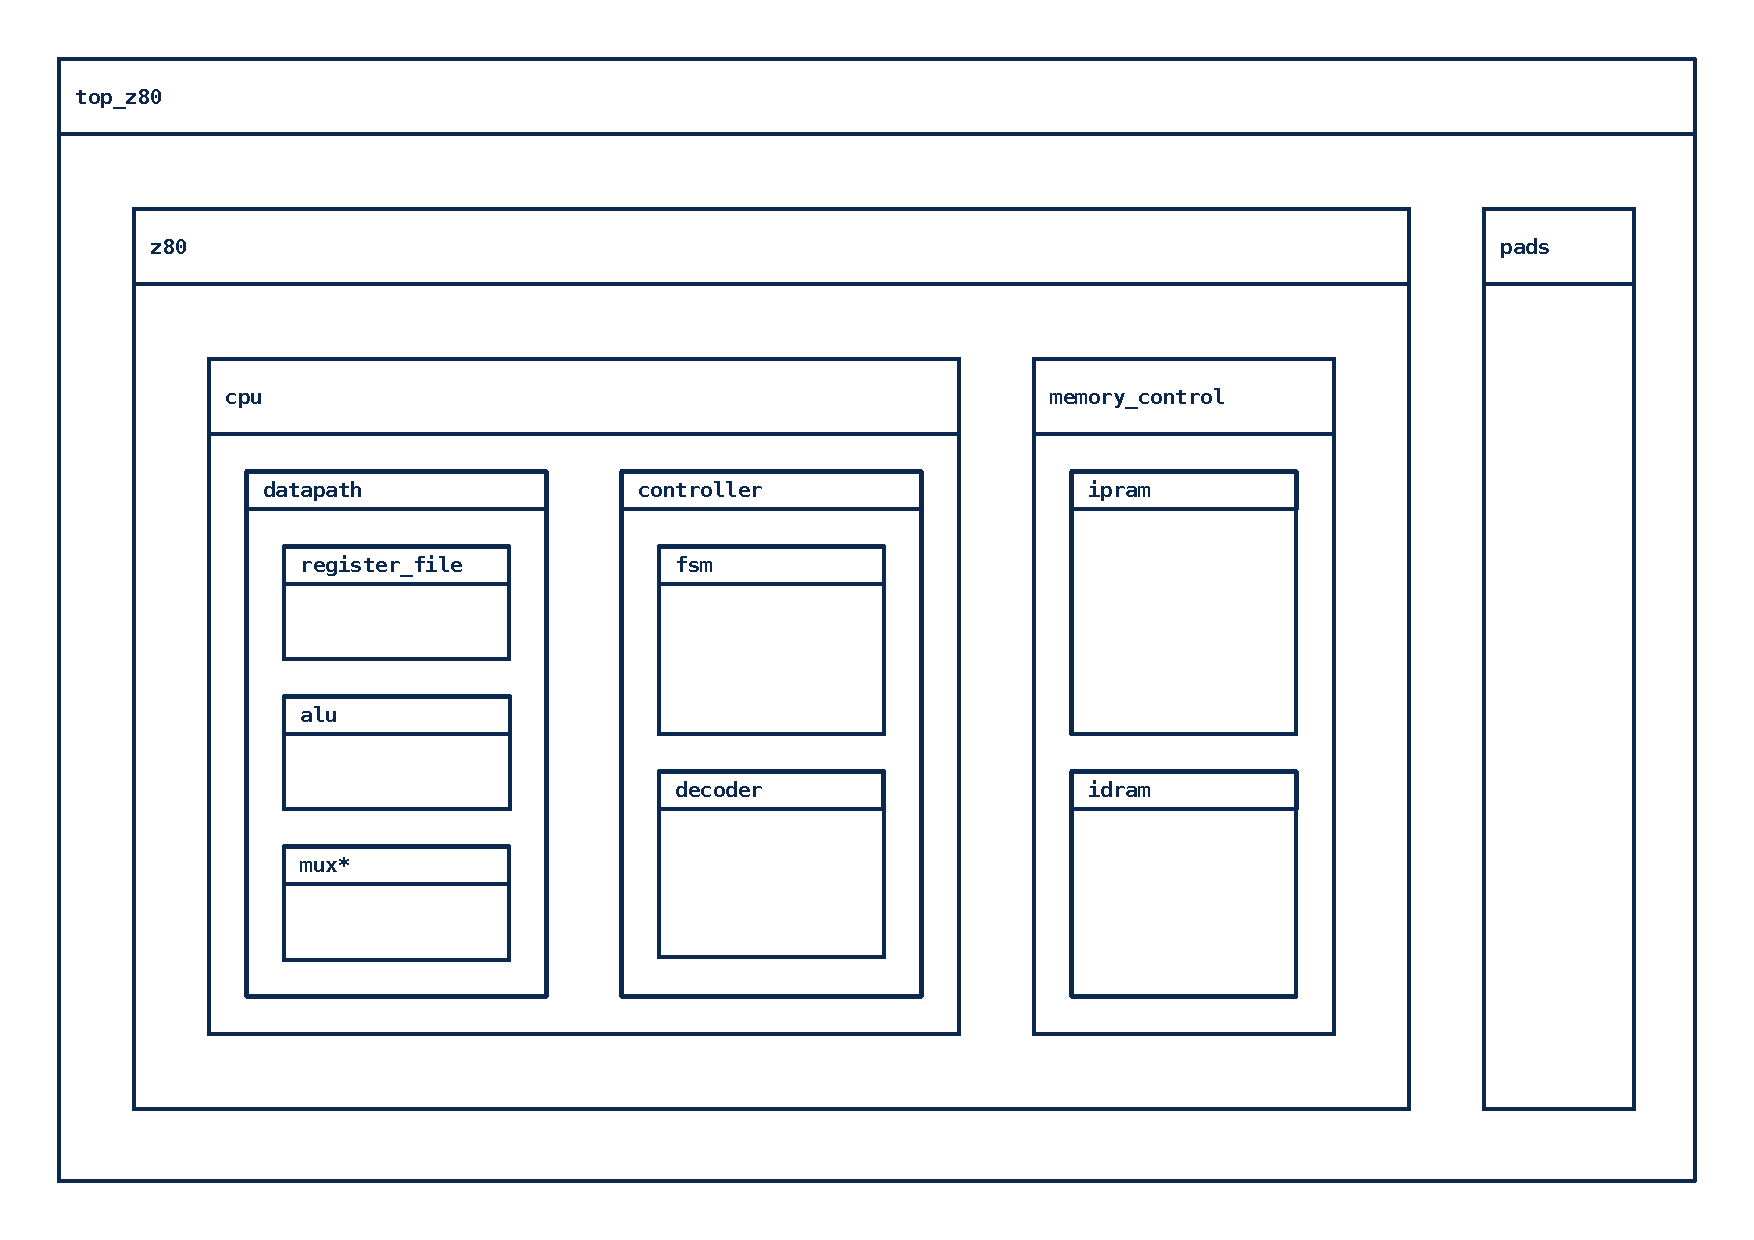
\includegraphics[width=.9\textwidth]{resources/pdf/module-structure.pdf}
  \caption{Modulstruktur}
  \label{img:module-structure}
\end{figure}

\noindent
Die Modulstruktur des Verilog Codes unserer Z80-Implementierung ist in
Abbildung~\ref{img:module-structure} gezeigt. Das Toplevel ist das Modul
\texttt{top\_z80}, in diesem sind der eigentliche Prozessor (Modul
\texttt{z80}) und die Pads instanziiert.

Das Modul \texttt{z80} enthält die CPU (Modul \texttt{cpu}) und die
Speicherverwaltung (Modul \texttt{memory\_control}). Alle Speicherzugriffe der
CPU werden an die Speicherverwaltung weitergeleitet. Diese spricht wiederum das
korrekte Speicherelement an. Der interne Programm- und der interne
Datenspeicher sind in den Modulen \texttt{ipram} und \texttt{idram}
implementiert, welche dünne Wrapper um die verwendeten proprietären
Speicher-Zellen sind. Beide sind im \texttt{memory\_control} Modul
instanziiert.

Die CPU besteht aus dem Datenpfad (Modul \texttt{datapath}) und einem
zugehörigen Controller (Modul \texttt{controller}), welcher die Steuersignale
für den Datenpfad generiert.

Die wichtigsten Elemente im Datenpfad sind das Register File (Modul
\texttt{register\_file}) und die ALU (Modul \texttt{alu}). Das Register File
kapselt die 8- und 16-Bit CPU-Register, die ALU implementiert alle
arithmetisch-logischen Operationen und die Generierung der Flags.

Der Controller besteht aus der FSM (Modul \texttt{fsm}) und dem Decoder (Modul
\texttt{decoder}). Die FSM ist der Zustandsautomat des Prozessors, der den
Ablauf der Befehlsabarbeitung koordiniert. Der Decoder generiert unter Kenntnis
des aktuellen Zustandes und der auszuführenden Instruktion kombinatorisch die
benötigten Steuersignale für den Datenpfad.

Fast alle Module binden per \texttt{`include} Statements ``Header-Files'' ein,
in denen von mehreren Modulen geteilte lokale Parameter definiert sind.
Lediglich die Busbreiten von Modul Ein- und Ausgängen sind in der Datei
\texttt{buswidth.v} der Einfachheit halber über \texttt{`define} Statements
global definiert.

Die folgenden Modulbeschreibungen beziehen sich bewusst auf den Stand der
Implementierung vor dem finalen Optimierungsschritt, welcher hierdurch besser
nachvollziehbar wird. Das heißt, dass die Beschreibungen an einigen wenigen
Stellen leicht vom eingereichten Verilog-Code abweichen können. Dies sollte die
Verständlichkeit der Ausführungen jedoch nicht beeinträchtigen. Die im finalen
Optimierungsschritt vorgenommenen Änderungen werden dann im
Abschnitt~\ref{ch:syn} erläutert.

\section{CPU}

Das \texttt{cpu} Modul ist das ``Herz'' der Implementierung. Prinzipiell ist
dieses Modul die eigentliche Implementierung der Dokumentation, Memory Control
und Pads stellen lediglich die Schnittstellen zu On-Chip Speicher und zur
``Außenwelt'' dar.

\subsection{Datenpfad}

\begin{figure}[htbp]
  \centering
    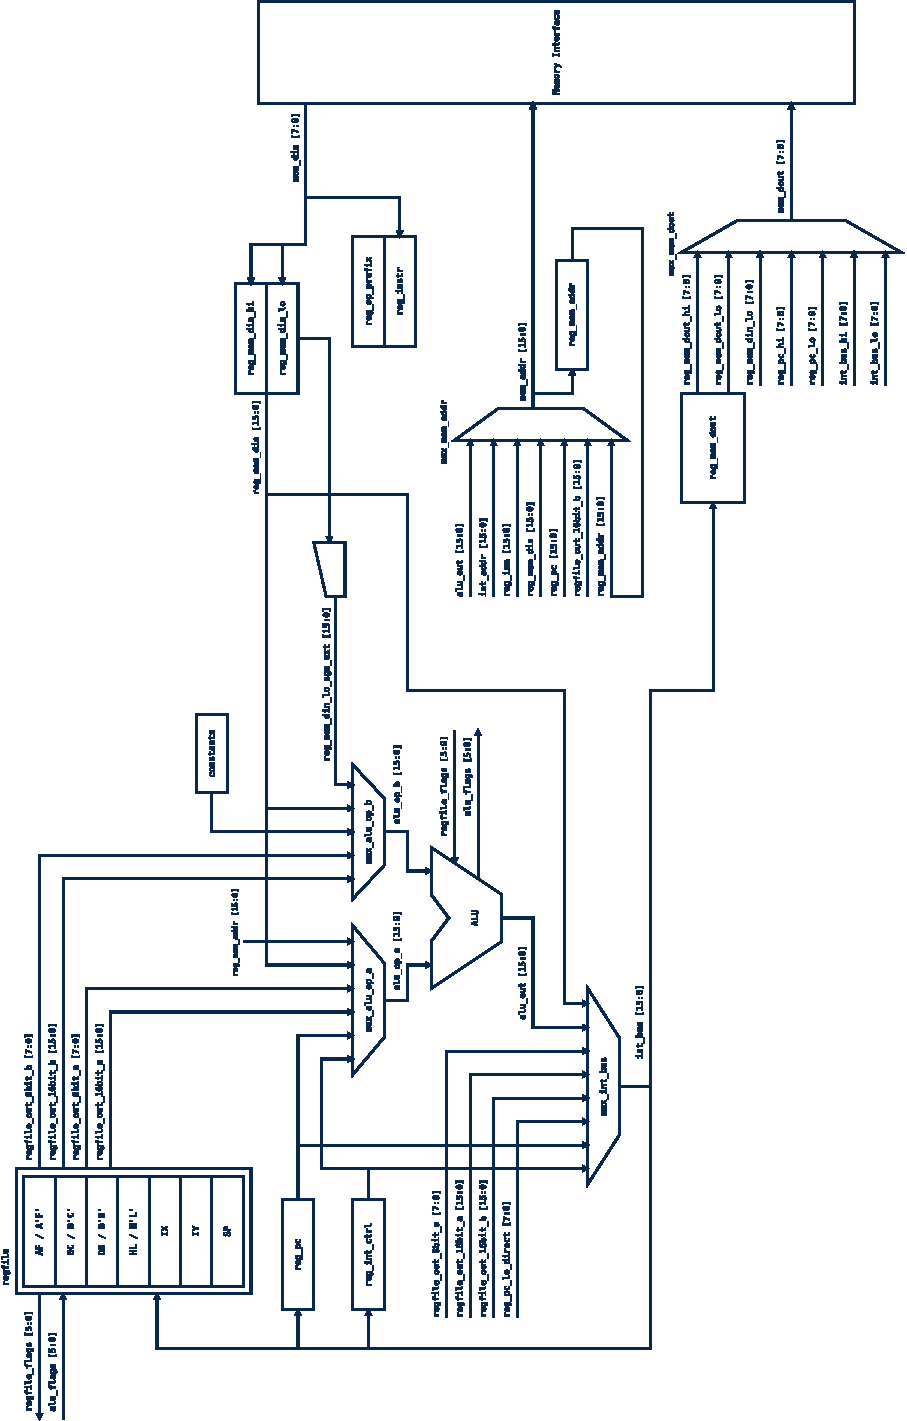
\includegraphics[height=\textheight]{resources/pdf/datapath.pdf}
  \caption{Datenpfad}
  \label{img:data-path}
\end{figure}

Abbildung~\ref{img:data-path} zeigt den schematischen Aufbau des Datenpfades.
ALU and Register-File werden in eigenen Abschnitten im Detail erläutert.

Im Datenpfad sind neben Register-File und ALU eine Reihe alleinstehender
Register, sowie mehrere Multiplexer instanziiert. Die alleinstehenden Register
sind alle Instanzen des \texttt{ff} Moduls, welches einen einfachen D-Flipflop
beschreibt.

Zu jedem Multiplexer existiert hingegen ein eigenes Modul. Einige der in
Abbildung~\ref{img:data-path} als Multiplexer-Eingänge dargestellten Signale
werden dabei teilweise erst in diesen Multiplexer-Modulen aus anderen Signalen
zusammengesetzt. Dies ist in Listing~\ref{lst:mux-alu-op-b} am Beispiel des
Mutiplexers für den ALU-Operanden B gezeigt. Unter anderem können der
konkatenierte Inhalt der beiden Dateneingangs-Puffer \texttt{reg\_mem\_din\_hi}
und \texttt{reg\_mem\_din\_lo}, der vorzeichenerweiterte Wert des
\texttt{reg\_mem\_din\_lo} Puffers oder der konstante Wert zwei (oft zur
Inkrementierung des PC vor dessen Ablage auf dem Stack benötigt) ausgegeben
werden.

\vskip\baselineskip

\noindent
\begin{minipage}{\linewidth}
\captionof{listing}{%
Alu-Operand B Multiplexer (\texttt{mux\_alu\_op\_b.v})
\label{lst:mux-alu-op-b}}
\inputminted[label=aluv]{verilog}{resources/verilog/mux-alu-op-b.v}
\end{minipage}

\vskip\baselineskip

\noindent
Der \texttt{data\_select} Eingang ist 1-aus-n kodiert, daher kann das
Ausgangs-Signal mit der gezeigten Kaskade von \texttt{if}-Statements selektiert
werden. Dies ist gerade bei Multiplexern, die zum kritischen Pfad gehören,
wichtig, da die Propagierung von Signalen durch den synthetisierten Multiplexer
so leicht beschleunigt wird (siehe auch Abschnitt~\ref{ch:syn}). Da der
entstehende Flächen-Overhead vernachlässigbar ist, wurde diese Optimierung der
Einfachheit halber in allen Multiplexer Modulen vorgenommen.

Wesentliches Merkmal des Datenpfades ist der interne 16-Bit Bus
\texttt{int\_bus}. Über den \texttt{mux\_int\_bus} Multiplexer können unter
anderem alle Register aus dem Register-File und die Ausgabe der ALU auf diesem
Bus ausgegeben und folgend in eines der Register des Register-Files, den
Program Counter, das Interrupt Control Register oder den 16-Bit
Datenausgabe-Puffer \texttt{reg\_mem\_dout} übernommen werden. Getrennte
Multiplexer sind hier nicht notwendig, da diese Register nie im gleichen Takt
beschrieben werden.  8-Bit Werte (zum Beispiel das Ergebnis einer 8-Bit
ALU-Operation) werden im unteren Byte des internen Datenbusses transportiert.

Der Multiplexer-Eingang \texttt{reg\_pc\_lo\_direct} wird vom Decoder während
nicht-maskierbarer Interrupts, maskierbarer Interrupts bei gesetztem
Interrupt-Modus 1 und RST Instruktionen auf das untere Byte der (konstanten)
Adresse gesetzt, zu der folgend gesprungen werden muss (das obere Byte
dieser Sprungadressen ist in jedem Fall null).

Zu beachten ist, dass es keine separaten arithmetischen Elemente zur
Inkrementierung des Program Counters oder zur Inkrementierung bzw.
Dekrementierung des Stack Pointers gibt, diese Aufgaben übernimmt die
ALU\footnote{Das 16-Bit Register \texttt{BC} kann jedoch auch ohne die ALU
dekrementiert werden, mehr dazu in Abschnitt~\ref{ch:regfile}.}.

Aus dem Register-File können parallel zwei beliebige 8- sowie 16-Bit Register
ausgelesen werden. Es werden in keinem Fall im gleichen Takt sowohl ein 8- als
auch ein 16-Bit Register benötigt, die Trennung der Register-File Ausgänge
``a'' und ``b'' in 8- und 16-Bit Varianten ist lediglich eine
Performance-Optimierung, welche die kombinatorische Verzögerung durch das
synthetisierte Register-File bei der Register-Auswahl reduziert.

Die ALU führt 8- und 16-Bit Datenoperationen aus, unter anderem Addition,
Subtraktion, Setzen und Löschen von Bits sowie Schiebeoperationen.
Die Operanden einer ALU-Operation werden über die Multiplexer
\texttt{mux\_alu\_op\_a} und \texttt{mux\_alu\_op\_a} an die ALU angelegt.
Einige ALU-Operationen verwenden dabei nur einen dieser Operanden.

Die ALU arbeitet prinzipiell immer mit 16-Bit Operanden und gibt ein
entsprechendes 16-Bit Ergebnis aus. Für 8-Bit Operationen werden nur die
unteren Bytes beider Operanden genutzt und nur das untere Byte des Ergebnisses
verwertet.

Der Inhalt des Flag-Registers liegt permanent über den \texttt{regfile\_flags}
Bus an der ALU an. Während jeder ALU-Operation werden die aktualisierten Flags
über den \texttt{alu\_flags} Bus ausgegeben, der wiederum Eingang des
Register-Files ist. Ist ein entsprechendes Kontrollsignal gesetzt, wird dieser
Wert mit steigender Taktflanke ins Register-File übernommen.

Die Kombination von internem 16-Bit Bus und 16-Bit ALU (im Gegensatz zur
Nutzung einer entsprechenden 8-Bit ALU) erlaubt es unter anderem, 16-Bit
ALU-Operationen und Adressberechnungen in nur einem Takt auszuführen, auf
Kosten einer größeren kombinatorischen Verzögerung durch die ALU in der
synthetisierten Schaltung.

\subsubsection{Speicher-Interface}

Die drei Busse, die die Schnittstelle zwischen Datenpfad und Speicher bzw.
externen Geräten darstellen, sind in Abbildung~\ref{img:data-path} mit dem mit
\textit{Memory-Interface} beschrifteten Block (der keinem Modul entspricht)
verbunden.

Beim lesenden Speicherzugriff wird die Adresse, von der gelesen werden soll, über
den \texttt{mux\_mem\_addr} Multiplexer auf den \texttt{mem\_addr} Bus
ausgegeben. Da diese hierbei stets über mehrere Takte gehalten werden muss
(siehe auch Abschnitt~\ref{ch:timing}), ist hinter den Multiplexer das Register
\texttt{reg\_mem\_addr} geschaltet, das wiederum ein Eingang des Multiplexers
ist. In einem typischen Anwendungsfall kann so in einem Takt eine von der ALU
berechnete Adresse auf \texttt{mem\_addr} ausgegeben und gleichzeitig mit der
nächsten steigenden Taktflanke in \texttt{reg\_mem\_addr} übernommen werden. In
folgenden Takten kann dann der Wert in \texttt{reg\_mem\_addr} zur
Speicher-Adressierung genutzt werden, während die ALU andere Operationen
ausführt.

Das Signal \texttt{int\_addr}\footnote{Achtung bei der Namensgebung: viele im
Zusammenhang mit Interrupt-Behandlung stehenden Signale haben den Präfix
``\texttt{int}'' mit dem internen Datenbus \texttt{int\_bus} als einiziger
Ausnahme.} wird im Multiplexer generiert und bei Auftreten von Interrupts im
Interrupt-Modus 2 genutzt. Das Signal setzt sich aus dem Wert des
\texttt{reg\_int\_ctrl} Registers und dem extern eigelesenen, in
\texttt{reg\_mem\_din\_lo} gepufferten unteren Byte der
Interrupt-Handler-Adresse zusammen (das niederwertigste Bit wird dabei immer
genullt um 16-Bit Alignment dieser Adresse zu garantieren).

Das Signal \texttt{reg\_imm} wird ebenfalls im Multiplexer generiert und setzt
sich aus dem Wert des Akkumulators (über \texttt{regfile\_out\_8bit\_b}) und
einem aus dem Speicher gelesenen Immediate Byte zusammen. Es wird während den
Instruktionen \texttt{IN A,(n)} und \texttt{OUT (n),A} zur Adressierung von
Geräten benötigt.

Wird während eines Instruction Fetches ein Opcode aus dem Speicher gelesen,
wird dieser im \texttt{reg\_instr} Register gespeichert. Viele Instruktionen
haben zusätzlich einen -maximal zwei Byte langen- \textit{Präfix}, der die
Bedeutung des Opcodes verändert. Der Decoder erkennt während eines
Instruction Fetch automatisch, dass das geladene Byte einen solchen Präfix
darstellt und dieser wird im Register \texttt{reg\_op\_prefix} festgehalten.
Dieses kodiert dabei auf kompakte Art sowohl ein- als auch zwei-Byte Präfixe.
Ein eingelesenes Präfix-Byte kann demnach nicht einfach in das Register
übernommen werden.  Stattdessen muss vom Decoder ein entsprechender neuer Wert
anhand des eingelesenen Präfix-Bytes und eines möglicherweise bereits in
\texttt{reg\_op\_prefix} kodierten, zuvor eingelesenen, Präfix-Bytes bestimmt
werden.  Die Inhalte beider Register werden an den Controller weitergereicht,
der sie nutzt um Entscheidungen bezüglich Zustandsübergängen und der Erzeugung
von Kontrollsignalen zu treffen.

Eingelesene Datenbytes werden hingegen in einem der Register
\texttt{reg\_mem\_din\_hi} und \texttt{reg\_mem\_din\_lo} gepuffert. Beim Lesen
von 16-Bit Werten aus dem Speicher in zwei aufeinanderfolgenden Leseoperationen
kann das höherwertige Byte in \texttt{reg\_mem\_din\_hi} und das niederwertige
Byte \texttt{reg\_mem\_din\_lo} gepuffert werden. Der durch Konkatenation der
Register-Inhalte enstehende 16-Bit Wert kann dann direkt auf den internen Bus
ausgegeben oder als Operand an die ALU angelegt werden.

Zusätzlich kann auch der auf 16-Bit vorzeichenerweiterte Wert des
\texttt{reg\_mem\_din\_lo} Puffers (hier mit
\texttt{reg\_mem\_din\_lo\_sgn\_ext} bezeichnet) als Operand B an die ALU
angelegt werden. Während Instruktionen, die mit indizierter Adressierung
arbeiten, wird der entsprechende Offset in diesen Puffer geladen und direkt im
nächsten Takt vorzeichenerweitert zum Inhalt eines der Register \texttt{IX}
oder \texttt{IY} addiert. Das Ergebnis kann sofort zur Speicheradressierung
genutzt werden. Hierdurch wird ein zusätzlicher Maschinen-Zyklus eingespart,
in dem sonst lediglich eine Adressberechnung und kein Speicherzugriff
durchgeführt werden müsste.

Für schreibende Speicherzugriffe wird das zu schreibende Byte auf dem Bus
\texttt{mem\_dout} ausgegeben. Hier wird ebenfalls ein Puffer eingesetzt,
jedoch vor dem Datenausgangs-Multiplexer \texttt{mux\_mem\_dout}. In
diesem können über den internen Bus 16-Bit Werte (z.B. von der ALU berechnete)
gepeichert und dann in zwei aufeinanderfolgenden Takten in den Speicher
geschrieben werden.

\subsubsection{Register File\label{ch:regfile}}

\begin{figure}[htbp]
  \centering
    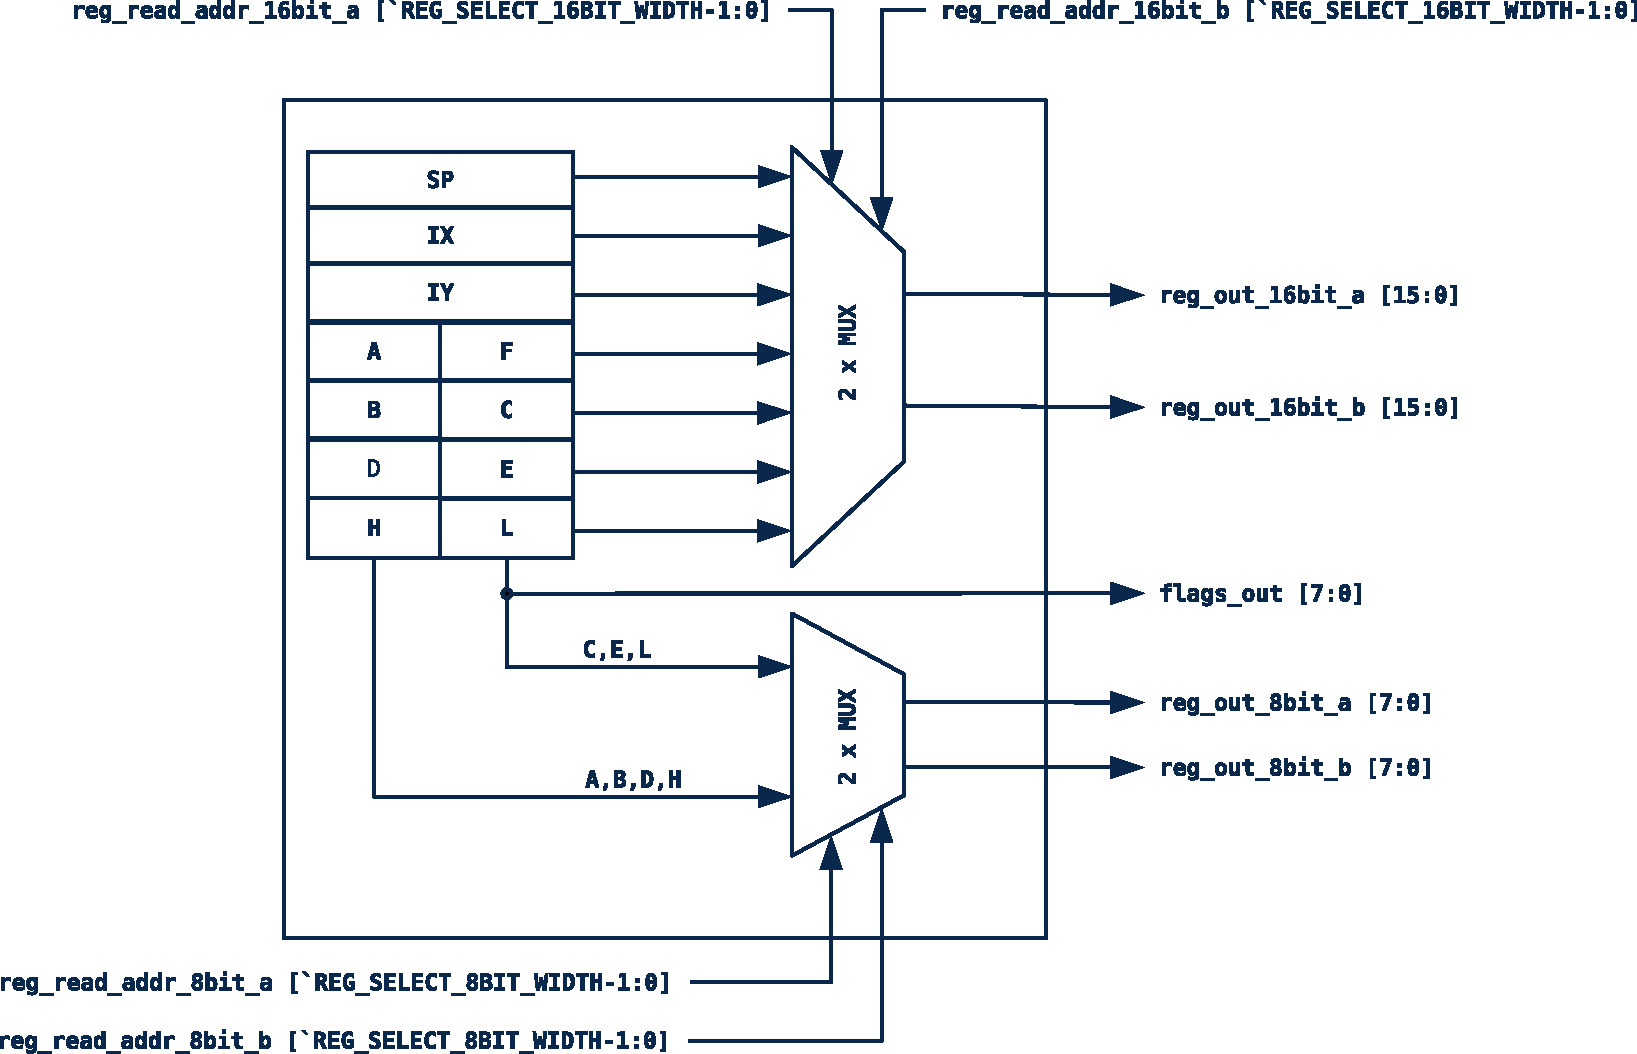
\includegraphics[width=\textwidth]{resources/pdf/regfile-read.pdf}
  \caption{Lesender Register-File Zugriff}
  \label{img:regfile-read}
\end{figure}

\noindent
Das Register File besteht aus drei 16-Bit Registern, acht 8-Bit Registern
sowie acht 8-Bit Schatten-Registern.

Abbildung~\ref{img:regfile-read} zeigt schematisch die für einen lesenden
Zugriff relevanten Komponenten des Register-Files. Das Flag-Register ist direkt
mit dem Ausgang \texttt{flags\_out} verbunden und somit permanent verfügbar.
Dabei werden die zwei undefinierten Flag-Bits des 8-Bit breiten Flag-Registers
nicht ausgegeben. Diese werden in unserer Implementierung auch nicht zum
Speichern temporärer Information o.ä. verwendet und können nicht direkt
beschrieben werden. Über die vier \texttt{reg\_read\_addr*} Eingänge kann
gesteuert werden, welche Register an den vier entsprechenden Ausgängen
ausgegeben werden. Die 8-Bit Register \texttt{A} und \texttt{F}, \texttt{B} und
\texttt{C}, \texttt{D} und \texttt{E}, \texttt{H} und \texttt{L} sind einzeln
als 8-Bit Register adressierbar, lassen sich aber auch paarweise über einen der
16-Bit Ausgänge ausgeben. Die Schattenregister lassen sich nicht auslesen und
sind in Abbildung~\ref{img:regfile-read} nicht gezeigt.

\begin{figure}[htbp]
  \centering
    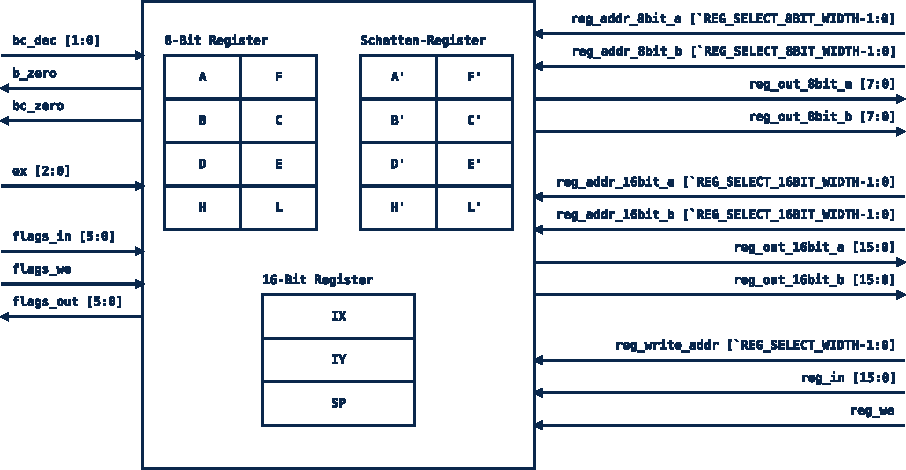
\includegraphics[width=\textwidth]{resources/pdf/regfile.pdf}
  \caption{Register-File}
  \label{img:regfile}
\end{figure}

\noindent
Abbildung~\ref{img:regfile} zeigt schematisch alle Register-File Ein- und
Ausgänge. Um ein Register zu beschreiben müssen die Daten an den 16-Bit
Eingang \texttt{reg\_in} angelegt werden. Das Zielregister für den
Schreibzugriff wird mit Hilfe des Signals \texttt{reg\_write\_addr} ausgewählt.
Im Gegensatz zu den \texttt{reg\_read\_addr*} Eingängen können über diesen
Eingang sowohl 8- als auch die 16-Bit Register angesprochen werden.  Ist der
Write-Enable-Eingang \texttt{reg\_we} aktiv, wird mit der nächsten steigenden
Taktflanke der anliegende Wert übernommen. Für 8-Bit Register ist dies stets
das untere Byte des an \texttt{reg\_in} anliegenden 16-Bit Wortes.  Für das
Flags-Register stehen der separate Eingang \texttt{flags\_in} und
Write-Enable-Eingang \texttt{flags\_we} zur Verfügung.

Weiterhin verfügt das Registerfile über einige besondere Funktionalitäten:

\begin{itemize}
\item
Der \texttt{regfile\_bc\_dec} Eingang wird während der Abarbeitung der
Block-Transfer- und Such-Instruktionen genutzt um ohne Nutzung der ALU den
Byte-Counter, d.h. das 16-Bit Register \texttt{BC} zu dekrementieren. Dadurch
müssen keine zusätzlichen Zustände ohne Speicherzugriff eingeführt oder
ALU-Operationen außerhalb des letzten Taktes eines Maschinen-Zyklus ausgeführt
werden (siehe auch Abschnitt~\ref{ch:decoder}).

Es wird hierfür zwischen zwei Modi unterschieden, \texttt{BC\_DEC\_LD} und
\texttt{BC\_DEC\_CP}. Der Eingang wird während der Instruktionen \texttt{LDI},
\texttt{LDIR}, \texttt{LDD} und \texttt{LDDR} auf ersteren gesetzt, während der
entsprechenden \texttt{CP*} Instruktionen auf letzteren. In beiden Fällen wird
das \texttt{BC} Register dekrementiert. Die Unterscheidung ist notwendig, da
gleichzeitig auch passende Änderungen am Flag-Register vorgenommen werden. Für
alle anderen Instruktionen wird der Eingang auf \texttt{BC\_DEC\_NONE} gesetzt.

\clearpage
\item
Der \texttt{regfile\_b\_zero} Ausgang des Register-Files ist immer dann
high wenn das 8-Bit Register \texttt{B} den Wert null hat. Er wird während der
\texttt{DJNZ} Instruktion genutzt um die Sprungentscheidung zu treffen.

\item
Der \texttt{regfile\_bc\_zero}  Ausgang des Register-Files ist
entsprechend dann high wenn das 16-Bit Register \texttt{BC} den Wert null hat
und wird während der Instruktionen \texttt{LDIR}, \texttt{LDDR}, \texttt{CPIR}
und \texttt{CPDR} gebraucht, die in diesem Fall abgebrochen werden können.

\item
Mit dem 1-aus-n kodierten \texttt{ex} Eingang kann in einem Takt der Inhalt von
Akkumulator und Flag-Register (\texttt{EX\_AF}) oder der \textbf{aller} 8-Bit
Register (\texttt{EX\_EXX}) mit dem der entsprechenden Schatten-Register
getauscht werden. Alternativ können auch 16-Bit Register \texttt{DE} und
\texttt{HL} vertauscht werden (\texttt{EX\_DE\_HL}). Damit können die
verschiedenen Exchange Intruktionen realisiert werden.
\end{itemize}

\subsubsection{ALU}

\begin{figure}[htbp]
  \centering
    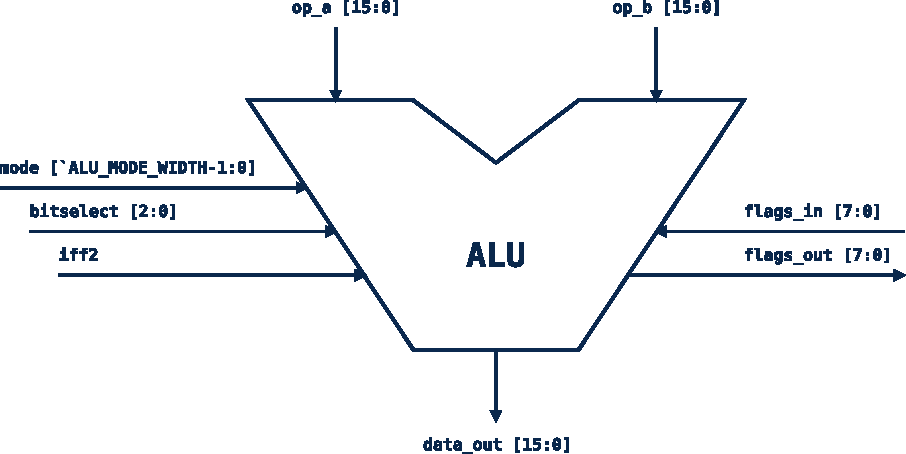
\includegraphics[width=0.7\textwidth]{resources/pdf/alu.pdf}
  \caption{ALU}
  \label{img:alu}
\end{figure}

\noindent
Abbildung~\ref{img:alu} zeigt schematisch alle Eingänge- und Ausgänge der ALU.
Über den \texttt{mode} Eingang kann der Controller die von der ALU
auszuführende Operation festlegen, dies beinhaltet auch die Generierung der
entsprechenden Flags, die wie zuvor beschrieben über \texttt{alu\_flags}
ausgegeben werden (nicht modifizierte Flags werden einfach von
\texttt{regfile\_flags} zu \texttt{alu\_flags} durchgereicht).  Einige wenige
Instruktionen modifizieren die Flags ohne eine damit zusammenhängende
ALU-Operation auszuführen, wie etwa die \texttt{IN} Instruktion, welche die
Flags allein in Abhängigkeit eines von einem externen Gerät eingelesenen Bytes
setzt. Für diese Fälle werden dennoch separate ALU-Modi definiert. Für die
genannte Instruktion muss hier z.B. das eingelesene Byte als Operand A an die
ALU angelegt werden und die ALU ist im gleichen Takt nicht für eventuell
parallel notwendige Berechnungen verfügbar. In unserem Design entstehen
hierduch jedoch an keiner Stelle Timing-Probleme.

Über den \texttt{bitselect} Eingang kann bei Bit-Set, -Reset und -Test
Operationen spezifiziert werden auf welchem der 8-Bits des Operanden A die
Operation ausgeführt werden soll.

Über den \texttt{iff2} Eingang liegt permanent der aktuelle Wert des
\texttt{iff2} Registers (im Modul \texttt{fsm} definiert) an der ALU an. Dieser
wird nur während der \texttt{LDAI} Instruktion benötigt, die außer der
Inkrementierung des PC keine ALU-Operation ausführt, aber den Wert von
\texttt{iff2} über \texttt{alu\_flags} als aktualisiertes Partitäts-Flag
ausgibt.

Alle arithmetischen ALU-Operationen werden intern über eine 16-Bit
Addierer-Beschreibung realisiert, die in Listing~\ref{lst:alu-adder} gezeigt
ist.  Für Subtraktionen nimmt \texttt{b} hierbei den invertierten Wert von
\texttt{op\_b} an. Der eingehende Carry \texttt{cin0} wird in Abhängigkeit
davon gesetzt, ob die auszuführende Operation eine Subtraktion beinhaltet und
ob diese das gesetzte Carry-Flag berücksichtigt.  Der Addierer setzt sich aus
mehreren Addierer-Beschreibungen variabler Bitbreite und zwei Full-Adder
Beschreibungen zusammen. Dies ist notwendig um eine Reihe von eingehenden und
ausgehenden Carries zu bestimmen. Anhand dieser werden für viele arithmetische
Operationen die resultierenden Carry- und Overflow-Flags bestimmt. Der
ausgehende Carry des dritten Bits, \texttt{cout3}, ist der Half-Carry bei 8-Bit
Additionen, bzw. das Inverse des Half-Borrows bei 8-Bit Subtraktionen.
\texttt{cout11} ist das Pendant für einige 16-Bit Operationen. Mit
\texttt{cin7} und \texttt{cout7} können Carry und Overflow für 8-Bit
Operationen, mit \texttt{cin15} und \texttt{cout15} für 16-Bit Operationen
bestimmt werden.

\vskip\baselineskip

\noindent
\begin{minipage}{\linewidth}
\captionof{listing}{%
16-Bit Adder Implementierung (Ausschnitt \texttt{alu.v}, angepasste Formattierung)
\label{lst:alu-adder}}
\inputminted[label=aluv]{verilog}{resources/verilog/alu-adder.v}
\end{minipage}

\vskip\baselineskip

\noindent
Logische, Shift- und Rotations- sowie Bit-Set/Reset Operationen sind mit
individuellen, weitestgehend selbsterklärenden Verilog-Statements implementiert.

Die ALU implementiert weiterhin die \texttt{DAA} Operation. Diese ist dabei
prinzipiell durch eine Reihe von Fallunterscheidungen realisiert, welche
in Ahängigkeit der eingehenden Flags und des Wertebereiches des als
Operand A angelegten Akkumulators-Inhaltes dessen korrigierten Wert bestimmen.
Die \texttt{DAA}-Instruktion kann dabei in einem Takt abgearbeitet werden. alle
möglichen Korrekturfaktoren sind als Konstanten im Source-Code der ALU
spezifiziert.

Nehmen Akkumulator und Flag-Register vor Ausführung der \texttt{DAA}
Instruktion Werte an, die im Kontext von \texttt{BCD}-Rechnungen so nicht
auftreten sollten, ist das Ergebnis laut Dokumentation undefiniert.  Wir haben
uns entschieden das Verhalten der \texttt{DAA} Operation in diesem Fall exakt
dem der \texttt{DAA} Instruktion anzupassen, die im von uns während
Verifikation verwendeten \texttt{z80sim} Software-Simulator implementiert ist.
Die Hardware-Beschreibung ist hierdurch komplizierter als unbedingt notwendig,
aber dafür wird die automatisierte Test-Generierung erleichtert (siehe
Abschnitt~\ref{ch:verification}).

\subsection{Controller}

Der Controller kapselt FSM und Decoder. In diese beiden Module ist der größte
Entwicklungsaufwand geflossen und ihre große Komplexität rechtfertigt
ihre Trennung.

\subsubsection{FSM}

Die Aufgabe der Finite State Machine besteht in der Koordinierung des Ablaufs
der Befehlsausführung. Der aktuelle Zustand wird intern in einem Register
gespeichert und über den Ausgang \texttt{state} dem Decoder zur Verfügung
gestellt. Der Folgezustand wird kombinatorisch in Abhängigkeit vom aktuellen
Zustand, Opcode-Präfix und Opcode bestimmt und mit der nächsten positiven
Taktflanke übernommen. Abbildung~\ref{img:fsm-states} zeigt den vereinfachten
Zustandsübergangsgraphen der FSM, in dem für jeden möglichen Zustandsübergang
eine Kante zwischen zwei Zuständen eingezeichnet ist. Dabei werden folgende
Abkürzungen genutzt:

\begin{description}[leftmargin=!,labelwidth=50px,itemsep=0pt]
  \item[IF:] Instruction Fetch
  \item[OF:] Operand Fetch
  \item[MR:] Memory Read
  \item[MW:] Memory Write
  \item[IOR:] IO Read
  \item[IOW:] IO Write
  \item[BT:] Block Transfer
  \item[AINT:] Interrupt Acknowledge
  \item[ANMI:] Non-maskable Interrupt Acknowledge
\end{description}

\begin{figure}
  \centering
    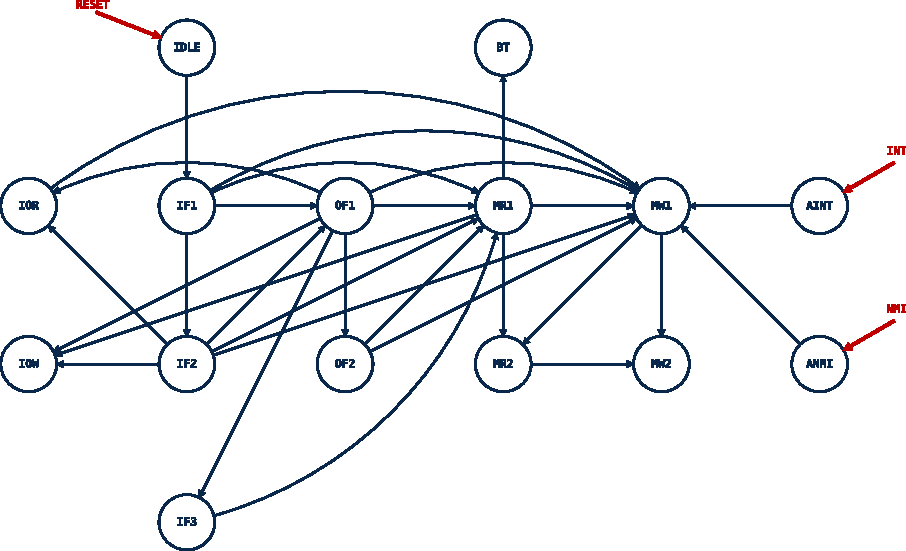
\includegraphics[width=\textwidth]{resources/pdf/fsm-states.pdf}
  \caption{Vereinfachter Zustandsübergangsgraph}
  \label{img:fsm-states}
\end{figure}

Die gezeigten Zustände entsprechen den Maschinen-Zyklen der Implementierung,
die wiederum mehrere Takte andauern können und demnach aus mehreren
Unterzuständen zusammengesetzt sind. Die möglichen Zustandsübergänge zurück zu
\texttt{IF1} sind der Übersichtlichkeit halber nicht dargestellt.

Nach einem initialen Reset befindet sich die FSM im \textit{Idle} Zustand und
verbleibt solange in diesem, bis der gesamte Programmspeicher von einer
externen Quelle eingelesen worden ist\footnote{Siehe Abschnitt~\ref{ch:ipram}}.
Danach wechselt die FSM in den ersten \textit{Instruction Fetch} Zustand
(\texttt{IF1}), der intern aus drei Unterzuständen \footnote{Im Verilog-Code in
diesem Fall durch die Konstanten \texttt{FSM\_STATE\_INSTR\_FETCH1\_1},
\texttt{FSM\_STATE\_INSTR\_FETCH1\_1\_2} und
\texttt{FSM\_STATE\_INSTR\_FETCH1\_3} identifiziert.} zusammengesetzt ist.  Ist
das in diesem Zustand eingelesene Byte ein Opcode-Präfix (oder ein Teil eines
solchen) folgt ein weiterer \texttt{Instruction Fetch} Zustand (\texttt{IF2}).

Anschließend erfolgt dann eine Reihe von Übergängen zwischen den übrigen
Zuständen, jeweils durch den über die Eingänge \texttt{reg\_instr} und
\texttt{reg\_op\_prefix} innerhalb der FSM verfügbaren Opcode und Opcode-Präfix
bestimmt. Listing~\ref{lst:fsm-verilog} zeigt einen relevanten
Code-Ausschnitt. Mittels des \texttt{casez} Statements können in Opcodes kodierte
Register o.ä. lesbar zusammengefasst werden. Für die Opcodes wurden keine
Mnemoniken eingeführt, da gleiche Opcodes in Abhängigkeit vom Opcode-Präfix
komplett unterschiedliche Bedeutungen annehmen können.

\vskip\baselineskip

\noindent
\begin{minipage}{\linewidth}
\captionof{listing}{FSM-Zustandübergangslogik (Ausschnitt \texttt{fsm.v})
\label{lst:fsm-verilog}}
\inputminted[label=aluv]{verilog}{resources/verilog/fsm-verilog.v}
\end{minipage}

\vskip\baselineskip

\noindent
Besonders hevorzuheben ist der \texttt{Block Transfer} Zustand (\texttt{BT}).
Dieser wird nur während der \texttt{CPIR} und \texttt{CPDR} Instruktionen
benötigt und ist außer dem \texttt{IDLE} Zustand der einzige, in dem kein
Speicher- oder IO Zugriff erfolgt. Dies ist die einzige Ausnahme zum in
Abschnitt~\ref{ch:design-goals} beschriebenen Prinzip der minimalen
Intruktions-Länge.

Die Interrupt Acknowledge \texttt{AINT} und Non-maskable Interrupt Acknowledge
Zustände (\texttt{AINT} und \texttt{ANMI}) werden nicht während der normalen
Befehlsabarbeitung, sondern erst nach Auftreten entsprechender Interrupts
erreicht. Die FSM übernimmt die Verwaltung des aktuellen Interrupt-Zustandes
und tastet Interrupt-Anfragen wie in der Dokumentation beschrieben mit der
steigenden Flanke des letzten Taktes jeder Instruktion ab.

Die Interrupt Control Flipflops \texttt{int\_iff1} und \texttt{int\_iff2} sind
dabei ebenfalls Teil der FSM und werden, wenn die Eingänge \texttt{int\_enable}
bzw. \texttt{int\_disable} aktiv sind, mit der nächsten steigenden Taktflanke
gesetzt bzw. zurückgesetzt. Das Umschalten des Interrupt-Modus sowie das
Wiederherstellen von \texttt{int\_iff1} nach Ende eines nicht maskierbaren
Interrupts sind ebenfalls in der FSM implementiert.

Im vorletzten Takt jeder Instruktion wird das interne \texttt{int\_sample}
Signal gesetzt. Ist dieses aktiv, werden mit der folgenden steigenden Flanke
des letzten Taktes der Instruktion die über \texttt{int\_request\_int} an der
FSM anliegenden Interrupt Requests gesampelt.

Ein nicht maskierbarer Interrupt Request hat dabei Priorität und hat das Setzen
des \texttt{int\_sampled\_nmi} Flipflops zur Folge. Für maskierbare Interrupts
wird das entsprechende \texttt{int\_sampled\_int} Flipflop nur dann gesetzt,
wenn auch das \texttt{int\_iff1} Flipflop gesetzt ist und im letzten Takt kein
Interrupt-Enable stattgefunden hat\footnote{Über den \texttt{int\_enable\_buf}
Flipflop realisiert.}.

Einen Sonderfall bilden die Instruction Fetches. Für diese ist erst nach dem
Einlesen des Bytes aus dem Programmspeicher entscheidbar, ob der Instruction
Fetch Maschinen-Zyklus der letzte der aktuellen Instruktion ist. Da das
Einlesen dieses Bytes mit dem Samplen der Interrupt Requests zusammenfällt,
musste hier das zusätzliche Signal \texttt{int\_suppress} eingeführt werden.
Bei Instruction Fetches werden die Interrupt Request immer gesampelt und
notfalls mit \texttt{int\_suppress} das Abarbeiten eines Interrupt-Requests
mitten in einer Instruktion unterdrückt.

Nach Auftreten eines Interrupts wechselt die FSM in den Interrupt-Acknowledge
oder den Non-maskable Interrupt Acknowledge Zustand und beginnt mit der in der
Dokumentation beschriebenen Interrupt-Behandlung. Währenddessen ist eines der
Signale \texttt{int\_active\_int} oder \texttt{int\_active\_nmi} aktiv, über
die FSM und Decoder z.B. im Memory Write Zustand, der Teil beider Interrupt
Acknowledge Vorgänge ist, erkennen können, dass spezielle Operationen
durchzuführen sind.

Der Interrupt Modus ist dabei im Register \texttt{int\_mode} in der FSM
gespeichert und wird an den Decoder weitergereicht. Interrupt Mode 0 ist nicht
vollständig implementiert, das Ausführen Instruktionen beliebiger Länge hätte
einen starken Eingriff in das bestehende Design erfordert. Außerdem gibt es
wenige realistischen Anwendungsfälle der Schaltung in denen Interrupt-Mode 0
nützlich wäre. Unsere Implementierung kann im Interrupt Modus 0 daher nur
ein-Byte Instruktionen ausführen.

\subsubsection{Decoder\label{ch:decoder}}

Der Decoder ist ein rein kombinatorisches Modul, welches in Abhängigkeit vom
aktuellen Zustand, der eingelesenen Instruktion sowie gesetzten Flags und dem
Interrupt-Zustand Kontrollsignale für alle Datenpfad-Elemente sowie Speicher-
und IO-Zugriffe generiert.

Zentrales Element der \texttt{decoder.v} Source-Datei ist ein
\texttt{case}-Statement, dessen Struktur die des im FSM Code-Ausschnitt in
Listing~\ref{lst:fsm-verilog} gezeigten \texttt{case}-Statements widerspiegelt.

Um Übersichtlichkeit zu wahren und dem Synthese-Compiler die Eliminierung
gemeinsamer Teilausdrücke zu erleichtern werden einige in mehreren Zuständen
identisch bestimmte Signale in einem separaten kombinatorischen
\texttt{always}-Block generiert. Dies betrifft Branch-Bedingungen (beispielhaft
in Listing~\ref{lst:cond-select} gezeigt) und im Opcode kodierte Register und
ALU-Modi.

\vskip\baselineskip

\noindent
\begin{minipage}{\linewidth}
\captionof{listing}{%
Dekodierung Branch-Bedingung (Ausschnitt \texttt{decoder.v})
\label{lst:cond-select}}
\inputminted[label=aluv]{verilog}{resources/verilog/decode-condition.v}
\end{minipage}

\vskip\baselineskip

\noindent
Fast alle Maschinen-Zyklen sind so strukturiert, dass erst in ihrem letzten
Takt in Abhängigkeit vom aktuellen Prozessorzustand Steuersignale generiert
werden, die die für die korrekte Ausführung der Instruktion nötigen
Datenoperationen in Bewegung setzen. In den vorangehenden Takten werden meist
nur Kontrollsignale für den Speicher- oder IO-Zugriff erzeugt, der mit wenigen
Ausnahmen in jedem Maschinen-Zyklus stattfindet. So werden zum Beispiel im
ersten Takt jedes Instruction Fetch nur Steuersignale für den Programmspeicher
erzeugt, im zweiten zusätzlich der PC inkrementiert und \texttt{reg\_instr}
oder \texttt{reg\_op\_prefix} beschrieben. Erst im dritten Takt werden je nach
eingelesenem Byte z.B. spezifische ALU-Operationen ausgeführt. Der relevante
Verilog-Code ist in Listing~\ref{lst:instr-fetch} gezeigt.

% This is a weird workaround to pygment not parsing verilog case-statements
% correctly

\definecolor{pygyellow}{RGB}{161,161,0}

\vskip\baselineskip

\noindent
\begin{minipage}{\linewidth}
\captionof{listing}{%
Struktur der Instruction Fetch Steuersignal-Generierung (Ausschnitt \texttt{decoder.v})
\label{lst:instr-fetch}}
\begin{minted}[escapeinside=||]{verilog}
case (state)
    |\textcolor{pygyellow}{FSM\_STATE\_INSTR\_FETCH1\_1,}|
    |\textcolor{pygyellow}{FSM\_STATE\_INSTR\_FETCH2\_1,}|
    |\textcolor{pygyellow}{FSM\_STATE\_INSTR\_FETCH3\_1:}|: begin
        mem_n_m1         = 1'b0;
        mem_n_pmem       = 1'b0;
        mem_n_mreq       = 1'b0;
        mem_n_rd         = 1'b0;
        mux_mem_addr_sel = MUX_MEM_ADDR_SEL_REG_PC;
    end
    |\textcolor{pygyellow}{FSM\_STATE\_INSTR\_FETCH1\_2,}|
    |\textcolor{pygyellow}{FSM\_STATE\_INSTR\_FETCH2\_2,}|
    |\textcolor{pygyellow}{FSM\_STATE\_INSTR\_FETCH3\_2:}| begin
        mem_n_m1         = 1'b0;
        mem_n_pmem       = 1'b0;
        mem_n_mreq       = 1'b0;
        mem_n_rd         = 1'b0;
        mux_mem_addr_sel = MUX_MEM_ADDR_SEL_REG_PC;

        alu_mode         = ALU_MODE_INC;
        mux_alu_op_a_sel = MUX_ALU_OP_A_SEL_REG_PC;
        mux_int_bus_sel  = MUX_INT_BUS_SEL_ALU_OUT;
        reg_pc_we        = 1'b1;

        reg_instr_we = 1'b1;
    end
    |\textcolor{pygyellow}{FSM\_STATE\_INSTR\_FETCH1\_3:}| begin

        // ...
\end{minted}
\end{minipage}

\vskip\baselineskip

\noindent
Ähnliches gilt für andere Maschinen-Zyklen. Dieses Vorgehen bietet sich an, da
z.B. für Maschinen-Zyklen, in denen ein Byte eingelesen wird, in den meisten
Fällen sowieso erst dann eine sinnvolle nächste Datenoperation durchgeführt
werden kann, wenn dieses Byte verfügbar ist, d.h. im letzten Takt des
Maschinen-Zyklus.

Die Speicher- und IO Steuersignale müssen in fast allen Fällen über mehrere
Takte eines Maschinen-Zyklus gehalten werden. Speicher-Adresse, Ausgangdaten
und einige andere Signale werden dabei immer bereits im letzten Takt des
vorhergehenden Maschinen-Zyklus generiert um das in Abschnitt~\ref{ch:timing}
beschriebene Timing-Verhalten zu erzeugen.

\section{Speicherverwaltung}

Die Hauptaufgabe der Speicherverwaltung ist es, eine Abstraktionsschicht für
Speicherzugriffe zu schaffen, deren nach außen (d.h. zur CPU hin) sichtbares
Verhalten im Einklang mit dem in der Dokumentation beschriebenen Speichermodell
ist (d.h. ein kontinuierlicher 16-Bit Adressraum in dem sowohl Programme als
auch Daten abgelegt sind).

Dadurch wird es unter anderem möglich unabhängig von der Implementierung
der CPU Änderungen an der konkreten Speicher-Architektur vorzunehmen.
Insbesondere existiert so die Trennung in externen Speicher und internen
Programm- bzw. Datenspeicher aus Sicht der CPU nicht.

Das \texttt{memory\_control} Modul kapselt dabei die \texttt{ipram} und
\texttt{idram} Module, welche wiederum dünne Wrapper um den verwendeten
internen Programm- und Datenspeicher sind.

Die Eingänge der Speicherverwaltung sind die von der CPU erzeugten
Speicher-Kontrollsignale, die alle ein externes Pendant haben \footnote{Mit
Ausnahme des \texttt{int\_n\_pmem} Signals, das aufgrund der internen Trennung
von Programm- und Datenspeicher notwendig ist um zwischen Zugriffen auf diese
zu unterscheiden.}.


Einige dieser Signale können einfach zum Toplevel hin durchgereicht werden.
Für \textoverline{\texttt{mreq}}, \textoverline{\texttt{rd}} und
\textoverline{\texttt{wr}} passiert dies jedoch nur dann, wenn auch tatsächlich
ein externer Speicherzugriff erforderlich ist, was anhand der anliegenden
Speicher-Adresse entschieden werden kann. Nach dem gleichen Prinzip wird für
lesende Operationen der korrekte Datenbus auf den \texttt{int\_dout} Ausgang
der Speicherverwaltung geschaltet, der mit dem Dateneingang der CPU verbunden
ist. Listing~\ref{lst:pmem-access} zeigt einen entsprechenden Code-Ausschnitt
für Zugriffe auf den Programmspeicher.

\vskip\baselineskip

\noindent
\begin{minipage}{\linewidth}
\captionof{listing}{%
Programmspeicherzugriff (Ausschnitt \texttt{memory\_control.v})
\label{lst:pmem-access}}
\inputminted[label=aluv]{verilog}{resources/verilog/pmem-access.v}
\end{minipage}

\vskip\baselineskip

\subsection{Interner Programmspeicher\label{ch:ipram}}

Das \texttt{ipram} Modul ist wiederum eine Abstraktionsschicht für den
verwendeten \texttt{SY180\_1024X8X4CM4} Speicher (im Folgenden mit
\textit{Speicher-Element} bezeichnet).

Nach jedem Reset des Chips wird der gesamte interne Programmspeicher aus einer
externen Quelle eingelesen. Im \texttt{ipram} Modul existiert zu diesem Zweck
ein 13-Bit Zähler, der bei einem Reset auf null gesetzt und anschließend mit
jeder steigenden Tatkflanke inkrementiert wird.

Solange die Initialisierung noch nicht abgeschlossen ist, ist auch das interne
\texttt{loaded} Signal nicht aktiv und Speicher-Element wird Takt für Takt und
Adresse für Adresse (von null beginnend) mit den jeweils am \texttt{din}
Eingang anliegenden Bytes gefüllt. Währenddessen ist der Chip-Enable Eingang des
Speicher-Elementes (\textoverline{\texttt{csb}}) kontinuierlich aktiv.

Schreibzugriffe auf das Speicher-Element erfolgen auf Basis von 32-Bit Worten.
Vier separate low-aktive write enable Eingänge (\texttt{bwe}) kontrollieren
welche der vier Bytes des am Schreibeingang des Speicher-Elementes anliegenden
32-Bit Wortes bei steigender Taktflanke tatsächlich übernommen werden. Einzelne
Bytes können somit in den Programmspeicher geschrieben werden, indem das am
Dateneingang des \texttt{ipram} Moduls anliegende Byte parallel an jedes der
vier Bytes dieses Schreibeinganges angelegt wird und die unteren beiden Bits des
Initialisierungs-Zählers genutzt werden um zu bestimmen, welches dieser Bytes
in einem gegebenen Takt geschrieben wird. Die verbleibenden Bits des Zählers
wählen das zu beschreibende 32-Bit Wort aus (\texttt{addr\_word}).

Erreicht der Initialisierungs-Zähler den Wert \texttt{13'b1000000000000} ist
das Speicher-Element vollständig geladen und das \texttt{loaded} Signal wird
aktiviert. Anschließend ist der Programmspeicher nur noch für lesende Zugriffe
verfügbar. Für diese wird auf ähnliche Weise anhand der unteren beiden Bits der
anliegenden Adresse entschieden, welches Byte des am Ausgang des
Speicher-Elementes anliegenden 32-Bit Wortes (\texttt{dout\_int}) vom
\texttt{ipram} Modul ausgegeben werden muss.

\vskip\baselineskip

\noindent
\begin{minipage}{\linewidth}
\captionof{listing}{%
Programmspeicher-Initialisierung (Ausschnitt \texttt{memory\_control.v})
\label{lst:pmem-init-internal}}
\inputminted[label=aluv]{verilog}{resources/verilog/pmem-init-internal.v}
\end{minipage}

\vskip\baselineskip

\noindent
Listing~\ref{lst:pmem-init-internal} zeigt den Verilog-Code, der das
beschriebene Verhalten implementiert. Die Verzögerung zu Beginn der zweiten
\texttt{always}-Schleife dient dazu, Timing-Warnungen im Simulator-Output zu
unterdrücken, die für das Synthese-Ergebnis nicht relevant sind.

Das \texttt{loaded} Signal wird außerdem von der Memory Control an die CPU
weitergereicht und signalisiert dieser, dass mit der Ausführung des geladenen
Programms begonnen werden kann.

\subsection{Interner Datenspeicher}

Der Aufbau des \texttt{idram} Moduls ist deutlich weniger kompliziert. Intern
sind in diesem zwei separate \texttt{SY180\_256X8X1CM8} Speicher-Elemente
instanziiert. Anhand der angelegten Adresse wird entschieden, welches dieser
beiden Speicher-Elemente aktiviert werden muss. Die unteren $2^8$ wählbaren
Adressen sind einem der Elemente zugeordnet, die restlichen $2^8$ Adressen dem
anderen.

\section{Toplevel und Pads}

Das Modul \texttt{z80} kapselt die Module \texttt{cpu} und
\texttt{memory\_control}. Die Pads sind in einem eigenen Modul (\texttt{pads})
implementiert und dieses ist im \texttt{top\_z80} Modul zusammen mit dem
\texttt{z80} Modul instanziiert.

Die Ausgänge des \texttt{z80} Moduls werden direkt durch Register getrieben um
die Stabilität dieser Signale zu garantieren. Die Werte der internen Speicher-
und IO Steursignale und Daten werden dabei zu jeder positiven Taktflanke
automatisch übernommen und liegen somit um einen Takt verzögert über die Pads
am Ausgang des Chips an.

Im \texttt{pad} Modul ist die in Listing~\ref{lst:dbus-pin} gezeigte, zum
externen Datenbus gehörige, Pad-Instanz hervorzuheben. Da sich ausgehende und
eingehende Daten-Bytes den gleichen externen Bus teilen, intern aber über die
getrennten Busse \texttt{data\_out} und \texttt{data\_in} von und zum Datenpfad
laufen, musste hier das (vom Decoder generierte) \texttt{data\_out\_en}
Kontrollsignal eingeführt werden. Ist dieses aktiv, wird das interne
\texttt{data\_out} Signal auf den externen Datenbus ausgegeben, andernfalls
nimmt das interne \texttt{data\_in} Signal den Wert des externen Datenbus an.

\vskip\baselineskip

\noindent
\begin{minipage}{\linewidth}
\captionof{listing}{%
IO-Pad Instanz für den externen Datenbus (Ausschnitt \texttt{pads.v})
\label{lst:dbus-pin}}
\inputminted[label=aluv]{verilog}{resources/verilog/dbus-pin.v}
\end{minipage}

\vskip\baselineskip

\chapter{Timing\label{ch:timing}}

Im Folgenden wird anhand einiger repräsentativer Waveforms das von unserer
Implementierung gezeigte Timing-Verhalten relevanter Steuersignale bei internen
und externen Speicher- und Gerätezugriffen sowie Interrupt-Ackknowledgements
und nach \texttt{HALT} Instruktionen aufgezeigt. Dieses unterscheidet sich im
Wesentlich durch die Anforderung, alle Steuersignale nur an positiven
Taktflanken umzuschalten, von der Dokumentation.

\begin{figure}[htbp]
  \centering
    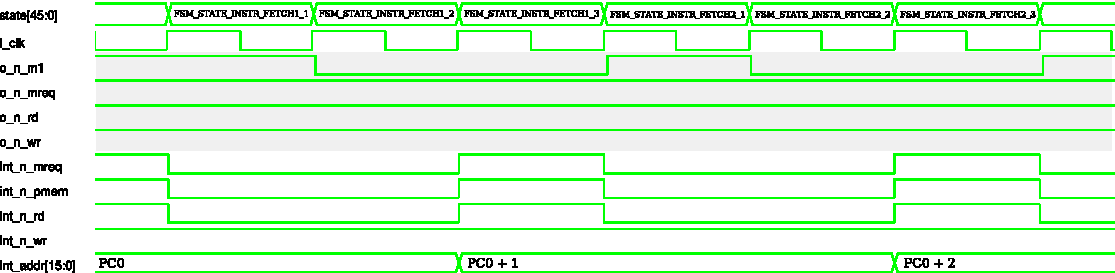
\includegraphics[width=\textwidth]{resources/pdf/prog-read.pdf}
  \caption{Interner lesender Programmspeicher-Zugriff}
  \label{img:prog-read}
\end{figure}

\noindent
In Abbildung~\ref{img:prog-read} ist das Steuersignal-Timing für das Auslesen
zweier Bytes aus dem internen Programmspeicher dargestellt. Die
\texttt{int*}-Signale sind Eingänge des \texttt{memory\_control} Moduls,
welches -unter anderem in Abhängigkeit der angelegten Speicher-Adresse- die
passenden Kontrollsignale für den internen Programmspeicher generiert oder
alternativ die Anfrage durch Erzeugung passender externer Kontrollsignale an
ein off-chip Speicherelement weiterleitet. Letztere Signale sind (grau
unterlegt) ebenfalls dargestellt.

Zu erkennen ist, dass die internen Steuersignale jeweils in den ersten zwei
Takten der drei Takte andauernden Leseoperationen aktiv sind. Dies ist
unbedingt notwendig, denn die entsprechenden externen Signale können nur mit
einer Verzögerung von einem Takt generiert werden, da diese direkt von
synchronen Registern im \texttt{z80} Modul getrieben werden, gleichzeitig aber
bei internen und externen Speicherzugriffen das eingelesene Byte an der
gleichen Taktflanke abgetastet werden muss\footnote{Hier die Flanke beim
Übergang vom jeweiligen zweiten zum dritten Takt.}. Andernfalls müssten interne
Komponenten der CPU wie Decoder und FSM ihr Verhalten abhängig davon, ob
aus dem internen oder externen Speicher gelesen werden soll, dynamisch anpassen.
Idealerweise sollte diesen Komponenten aber die Existenz eines einzigen
kontinuierlichen Adressraums vorgetäuscht werden, um sie robust gegenüber
Änderungen an der Speicher-Infrastruktur zu machen.

Die Speicheradresse wird bereits im jeweils letzten Takt des
\textbf{vorherigen} Maschinen-Zyklus angelegt, damit diese stabil ist, wenn
\texttt{int\_n\_mreq} bzw. \texttt{o\_n\_mreq} aktiv wird. Die Adresse wird
solange gehalten, bis das einzulesende Byte abgetastet worden ist.

Zu beachten ist weiterhin das \texttt{o\_n\_m1} Signal, welches in
Übereinstimmung mit der Dokumentation bei jedem Instruction Fetch (hier zwei in
Folge) aktiv wird, auch dann, wenn der eigentliche Zugriff auf den internen
Speicher erfolgt. Außerdem existiert das zusätzliche \texttt{int\_n\_pmem}
Steuersignal, welches durch die interne Trennung von Programm- und
Datenspeicher notwendig wird und dem \texttt{memory\_control} Modul bei
internem Speicherzugriff signalisiert, welcher von beiden angesprochen werden
muss.

\begin{figure}[htbp]
  \centering
    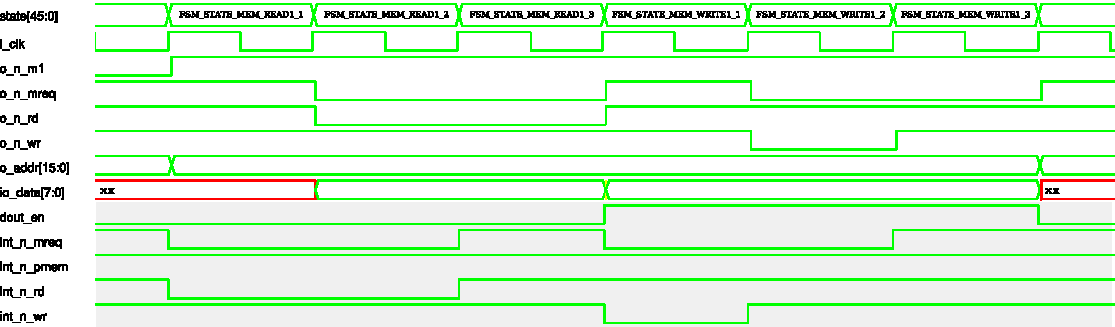
\includegraphics[width=\textwidth]{resources/pdf/mem-read-write.pdf}
  \caption{Externer lesender und schreibender Datenspeicher-Zugriff}
  \label{img:mem-read-write}
\end{figure}

\noindent
Abbildung~\ref{img:mem-read-write} zeigt das Steuersignal-Timing für einen
Lesezugriff gefolgt von einem Schreibzugriff auf den externen Speicher. Hier
ist nocheinmal die Verzögerung der externen gegenüber den internen Signalen
(hier grau unterlegt) verdeutlicht. Zusätzlich ist hier das Signal
\texttt{dout\_en} wichtig, welches durch Ansteuerung des entsprechenden IO-Pins
das zu schreibende Byte auf den externen tristate Datenbus ausgibt. Dieses wird
zusammen mit \texttt{dout\_en} analog zur Speicheradresse intern bereits im
jeweiligen Zustand vor \texttt{FSM\_STATE\_MEM\_READ*\_1} angelegt. Außerdem
ist zu beachten, dass das \texttt{int\_n\_wr} bzw. \texttt{o\_n\_wr} Signal
beim schreibenden Speicherzugriff nur in einem Takt aktiv ist, sodass Adresse
und Daten in Übereinstimmung mit der Dokumentation noch einen Takt nach
Deaktivierung von \texttt{n\_wr} stabil sind.

\begin{figure}[htbp]
  \centering
    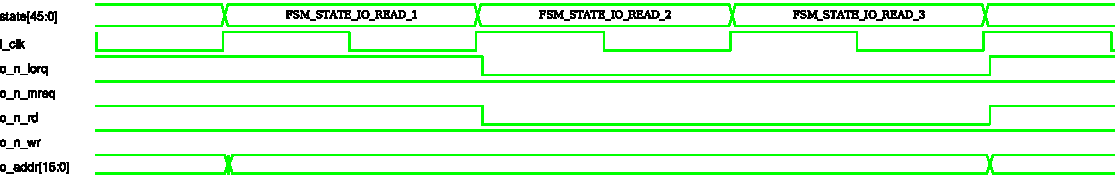
\includegraphics[width=\textwidth]{resources/pdf/io-read.pdf}
  \caption{IO Lesezugriff}
  \label{img:io-read}
\end{figure}

\begin{figure}[htbp]
  \centering
    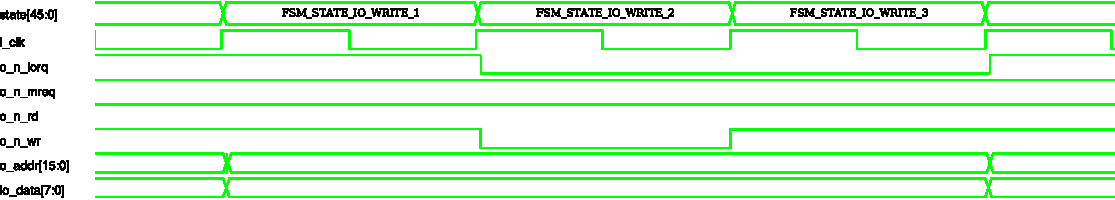
\includegraphics[width=\textwidth]{resources/pdf/io-write.pdf}
  \caption{IO Schreibzugriff}
  \label{img:io-write}
\end{figure}

\noindent
Abbildung~\ref{img:io-read} und Abbildung~\ref{img:io-write} zeigen die
relevanten Signalverläufe für lesende bzw. schreibende Zugriffe auf externe
Geräte. Diese sind selbsterklärend, \texttt{o\_n\_iorq} ersetzt hier
\texttt{o\_n\_mreq}.

\pagebreak

\begin{figure}[htbp]
  \centering
    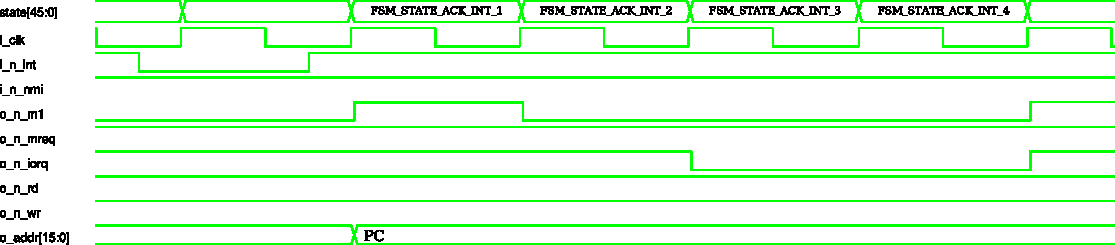
\includegraphics[width=\textwidth]{resources/pdf/ack-int.pdf}
  \caption{Interrupt Acknowledgement}
  \label{img:ack-int}
\end{figure}

\begin{figure}[htbp]
  \centering
    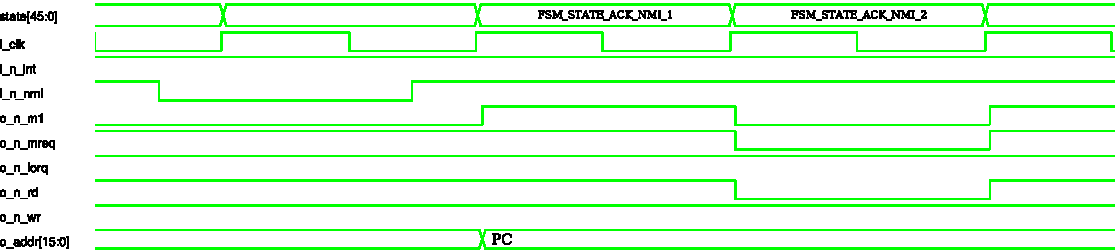
\includegraphics[width=\textwidth]{resources/pdf/ack-nmi.pdf}
  \caption{Non-maskable Interrupt Acknowledgement}
  \label{img:ack-nmi}
\end{figure}

\noindent
Abbildung~\ref{img:ack-int} und Abbildung~\ref{img:ack-nmi} zeigen die
Signalverläufe während der Interrupt Acknowledgements. Diese orientieren sich
an der Dokumentation. Speicher-Operationen wie das Ablegen des Program Counters
auf dem Stack, welche im Zuge eines Interrupt Acknowledgements durchgeführt
werden müssen\footnote{Im Falle eines maskierbare Interrupts in Abhängigkeit
vom eingestellten Interrupt-Modus.}, werden im Anschluss an die hier gezeigten
Zustände in gewöhnlichen \texttt{FSM\_STATE\_MEM\_WRITE*} etc. Zuständen
durchgeführt.

\begin{figure}[htbp]
  \centering
    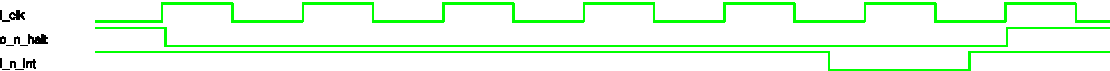
\includegraphics[width=\textwidth]{resources/pdf/halt.pdf}
  \caption{HALT}
  \label{img:halt}
\end{figure}

Abbildung~\ref{img:halt} zeigt den Effekt einer \texttt{HALT} Instruktion. Es
werden kontinuierlich No-Ops ausgeführt -wobei der \texttt{o\_n\_halt} Ausgang
aktiv ist- bis ein Interrupt (maskierbar oder nicht-maskierbar) auftritt und
abgehandelt wird.

\chapter{Verifikation\label{ch:verification}}

Einer der wichtigsten Schritte bei der Entwicklung einer komplexen digitalen
Schaltung ist die Verifikation von deren Korrektheit. Im Umfang dieser
Belegarbeit ist das letztendliche Ziel sicherzustellen, dass das simulierte
Verhalten der entworfenen Schaltung nach abgeschlossenem Layout-Schritt mit dem
dokumentierten Verhalten eines Z80 Prozessors übereinstimmt.

Im Folgenden werden die dabei von uns verfolgten Grundansätze und die zur
automatischen Testgenerierung und -ausführung verwendeten Methoden beschrieben.
Dabei wird immer wieder der Begriff \textit{Testfall} verwendet, der hier eine
\texttt{testcase.v} Datei im Kontext der von uns entwickelten Testumgebung
bezeichnet. Ein Testfall setzt sich dabei stets aus mehreren \textit{Tests}
zusammen, wobei jeder Test die Funktionalität einer Instruktion für einen
bestimmten Ausgangs-Systemzustand verifiziert.

\section{Grundansätze}

Bei der Entwicklung des Prozessors haben wir uns an dem in der
Software-Entwicklung weit verbreiteten Prinzip der \textit{Testgetriebenen
Entwicklung} (im Folgenden kurz \texttt{TDD}) orientiert.

Nachdem mit dem Entwurf eines Minimal-Prozessors eine grobe Modulstruktur
etabliert war, wurde bei der schrittweisen Implementierung jeder weiteren
Instruktion jeweils \textbf{bevor} die notwendigen Änderungen an FSM, Decoder
(und in manchen Fällen auch am Datenpfad) durchgeführt wurden, ein Testfall
angelegt, dessen Bestehen ein ausreichend guter Indikator für die korrekte
Funktionalität der neu hinzukommenden Instruktion ist. Anschließend wurde der
Verilog-Code jeweils bis zum Bestehen aller Tests in diesem Testfall
modifiziert. Erst danach wurden die entsprechenden Änderungen in die
Versionsverwaltung übernommen.

Dieses Vorgehen wurde strikt für alle implementierten Instruktionen
eingehalten. So konnte gewährleistet werden, dass zu keinem Zeitpunkt
fehlerhafte oder unvollständige Instruktionen in das Design übernommen wurden.
Zudem wurden in periodischem Abstand automatisiert alle bisher entwickelten
Test ausgeführt um durch Abhängigkeiten zwischen verschiedenen Instruktionen
oder Änderungen an von mehreren Instruktionen genutzten Elementen (wie zum
Beispiel dem Speichercontroller) entstandene Fehler rechtzeitig erkennen und
beheben zu können.

Wir haben uns in diesem Zusammenhang auch dafür entschieden, letztendlich nur
das nach außen für einen Anwender der resultierenden Schaltung sichtbare
Verhalten (welches bei korrekter Implementierung deckungsgleich mit dem in der
Dokumentation beschriebenen sein sollte) zu testen. Das Verhalten von
Untermodulen wie beispielsweise der ALU oder der FSM wurde bei deren initialer
Entwicklung durch eigene, speziell auf diese Komponenten abgerichtete Tests
überprüft. Im Verlauf des Projektes wurden alle derartigen Tests aber zugunsten
von Toplevel Tests, welche lediglich durch Instruktionen oder äußere Stimuli
hervorgerufene System-Übergänge testen, wieder entfernt. Der Gedanke hinter
dieser Entscheidung ist, dass das Verhalten der internen Komponenten letztlich
irrelevant ist, solange es nach außen hin den gewünschten Effekt hat.
Dieses nicht zu testen spart dabei wertvolle Entwicklungszeit und erhöht die
``Stabilität'' der Tests gegenüber internen Strukturänderungen.
Auch die genaue Ausführungszeit einzelner Instruktionen in Hinsicht auf
Maschinen-Zyklen und T-states wird nicht getestet, da diese in den meisten
Fällen in unserer Implementierung ohnehin gewollt von der dokumentierten
abweichen.

Dieses Vorgehen ist gemeinhin als \texttt{Black-Box-Testing} bekannt. Einzig
problematisch ist hierbei eventuelle fehlerhafte oder überflüssige
Funktionalität in Untermodulen, die sich nicht bis zum Toplevel fortpflanzt und
bei der angewandten Testmethodik somit unbemerkt bleibt. Durch Analyse der
durch die Tests erzeugten Code Coverage kann dieser Fall aber größtenteils
ausgeschlossen werden.

Ein weiteres Problem, vor das wir uns in Bezug auf die Test-Entwicklung bereits
bei der Entwicklung des Minimal-Prozessors gestellt sahen, ist die durch die
komplexe Befehlssatzarchitektur des Z80 bedingte riesige Menge an Tests, die
nötig sind um die korrekte Funktionalität aller Instruktionen in allen
erdenklichen Grenzfällen sicherzustellen. Eine erschöpfende Verifikation ist
von vornherein ausgeschlossen, da hierzu das Verhalten jeder Instruktion
jeweils für alle möglichen Prozessor- und Speicher-Ausgangszustände
sichergestellt werden müsste. Aber auch eine annehmbare Testabdeckung, welche
für jede Instruktion jeden relevanten Fall (z.B. das korrekte Setzen aller von
der Instruktion beeinflussten Flags) zumindest einmalig testet, ist ohne
automatisierte Erzeugung der Testfälle fast nicht erreichbar. Bei mehreren
hundert möglichen Instruktionen sollten schätzungsweise zumindest einige
tausende Tests nötig sein um eine derartige Testabdeckung zu erreichen. Das
Schreiben der Tests würde somit den Großteil der gesamten zur Verfügung
stehenden Entwicklungszeit beanspruchen, vor allem auch da so zusätzlich
äußerste Sorgfalt nötig ist um sicherzustellen, dass die Testfälle sowohl
vollständig als auch korrekt sind.

In diesem Zusammenhang steigt dann auch die Wahrscheinlichkeit, dass sich durch
menschliches Versagen Fehler in die Tests selbst einschleichen. Dies führt
wiederum zu erhöhtem Entwicklungsaufwand, da hierdurch bei der Diagnose der
Ursache fehlschlagender Tests sowohl Fehler in der Implementierung als auch
Fehler in den Tests selbst in Betracht gezogen werden müssen. Außerdem kann es
passieren, dass Fehler in der Implementierung unentdeckt bleiben, wenn
fehlerhafte Tests die gewünschte Verhaltensprüfung nicht oder nur teilweise
implementieren. Im schlimmsten Fall kann es auch dazu kommen, dass das im Test
geprüfte Verhalten zum Beispiel durch ein Missverständnis seitens des
Entwicklers zwar mit dem Verhalten der Implementierung, aber nicht mit dem in
der Dokumentation beschriebenen Verhalten übereinstimmt. Derartige Fehler in
der Implementierung bleiben dann mit großer Wahrscheinlichkeit ebenfalls
unentdeckt. Zudem wird dem Entwickler durch das Bestehen der zugehörigen
Testfälle ein falsches Gefühl der Sicherheit bezügliches des geprüften
Verhaltens vermittelt. Das Risiko solcher Fehler wird durch den Einsatz von
\texttt{TDD} verstärkt, da die Entwicklung der Implementierung sich hier wie
beschrieben gänzlich nach dem durch die Tests geforderten Verhalten richtet.

Ebenso wie das Schreiben von Tests ist auch deren Verifikation allein durch
individuelle Inspektion von simuliertem Waveform-Output nicht praktikabel,
sowohl aus Zeitgründen, als auch wegen der erneuten Möglichkeit menschlichen
Versagens bei der Auswertung.

Um diese beiden Problemstellungen -also das Erzeugen einer großen Menge
fehlerfreier Tests in kurzer Zeitspanne und deren effiziente und korrekte
Verifizierung- zu lösen haben wir bereits zu Beginn der Entwicklungsphase
Konzepte zur automatischen Testgenerierung und \mbox{-verifikation} entwickelt
und diese durch eine Reihe von Skripten umgesetzt, deren Funktionalität im
Verlauf des Projektes in Anpassung an neu hinzukommende Instruktionen stetig
verbessert und erweitert wurde und die letztendlich die Effizienz des
Entwicklungsprozesses drastisch gesteigert haben. Der folgende Abschnitt
beschreibt kurz die Implementierung der für alle Tests eingesetzten Testbench,
anschließend wird im Detail auf die Implementierung und Funktionalität dieser
Skripte eingegangen.

\section{Toplevel Testbench}

Alle Testfälle sind dem beschriebenen \texttt{Black-Box-Testing} Prinzip nach
für das \texttt{top\_z80} Modul implementiert. Somit wird mit jedem Test nicht
nur das korrekte Verhalten der CPU selbst sondern auch das der
Speicher-Kontrolllogik, des internem Programm- und Datenspeicher sowie der
IO-Pins getestet. Zusätzlich sind in der zugehörigen Testbench ein externer
Datenspeicher sowie ein ``IO-Speicher'' an die zu testende Schaltung
angeschlossen (siehe Listing~\ref{lst:mock-mem}).

Beide Speicher sind dabei durch das Modul \texttt{datamem\_mock}
modelliert, welches nicht in der synthetisierten Schaltung verwendet wird.
Dieses bietet ein einfaches Interface zum Schreiben und Auslesen von Daten
eines Speichers variabler Größe. Außerdem implementiert es einen einfachen
Plausibilitäts-Check für Speicherzugriffe. Dabei werden bei Schreib- und
Leseoperationen nur dann valide Daten geschrieben bzw. ausgegeben, wenn
die anliegende Speicheradresse mit der vor der letzten Aktivierung des
Chip-Enable Eingangs anliegenden Adresse übereinstimmt. Kompliziertere Fehler
wie das zu kurze Halten der Speicheradresse \textbf{nach} erfolgter
Schreiboperation werden an dieser Stelle nicht behandelt.

Durch den ``IO-Speicher'' werden externe Geräte modelliert. Dass bei Input- und
Output Instruktionen korrekte Daten ausgegeben und eingelesen werden, kann
mithilfe dieses Speichers einfach überprüft werden indem das \texttt{n\_iorq}
Signal als Chip-Enable für die entsprechende \texttt{datamem\_mock} Instanz
genutzt wird.

\vskip\baselineskip

\noindent
\begin{minipage}{\linewidth}
\captionof{listing}{%
Externer Datenspeicher und ``IO-Speicher'' (Ausschnitt \texttt{tb\_top\_z80.v})
\label{lst:mock-mem}}
\inputminted[label=aluv]{verilog}{resources/verilog/mock-mem.v}
\end{minipage}

\vskip\baselineskip

\noindent
Zusätzlich existieren in der Testbench ``Swap-Speicher'' für Daten- und
IO-Speicher. Diese Swap-Speicher werden benötigt, da während der
automatisierten Testfälle schreibende Speicherzugriffe nach jedem Test
rückgängig gemacht werden müssen. Andernfalls könnten Abhängigkeiten zwischen
den einzelnen Tests eines Testfalls entstehen, wenn in einem Test ein in einem
anderen geschriebenes Byte eingelesen wird. Dies sollte möglichst vermieden
werden um die Test-Generierung und letztlich auch das Debuggen fehlerhafter
Instruktionen durch Analyse der Testergebnisse zu erleichtern. Die
Swap-Speicher werden mit den gleichen Inhalten initialisiert wie die
tatsächlichen Speicher-Instanzen. Der Daten-Swap-Speicher wird dabei aus den
Inhalten des internen und externen Datenspeicher zusammengesetzt. Nach
einem schreibenden Speicherzugriff kann dann die beschriebene Stelle im
betroffenen Speicher mithilfe des entsprechenden Swap-Speichers zurückgesetzt
werden.

Vor Ausführung der Testfälle übernimmt die Testbench zudem die Initialisierung
des Programmspeichers mittels des von uns dafür vorgesehenen Mechanismus. Dazu
wird der Inhalt des internen Programmspeichers zunächst in ein
Hilfs-Speicherelement in der Testbench geladen. Anschließend wird dieser Byte
für Byte an den Datenbus-Eingang des Chips angelegt (nach Deaktivierung des
Reset-Signals). Nachdem der interne Programmspeicher eingelesen ist beginnt die
CPU automatisch mit der Ausführung des geladenen Programms (siehe
Abschnitt~\ref{ch:ipram}). Der relevante Code ist in
Listing~\ref{lst:pmem-init} gezeigt.

\vskip\baselineskip

\noindent
\begin{minipage}{\linewidth}
\captionof{listing}{%
Initalisierung des internen Programmspeichers (Ausschnitt \texttt{tb\_top\_z80.v})
\label{lst:pmem-init}}
\inputminted[label=aluv]{verilog}{resources/verilog/pmem-init.v}
\end{minipage}

\vskip\baselineskip

\noindent
Die Ausgänge von externem Daten- und IO-Speicher sowie dem
Initialisierungs-Signal sind alle mit dem Datenbus-Eingang des Chips verbunden,
nach Abschluss der Initialisierung geht letzteres in einen High-Impedance
Zustand über (ebenso die Speicher wenn der entsprechende Chip-Enable Eingang
nicht aktiv ist).

\section{Automatische Testgenerierung}

Inspiration für die automatisierte Generierung von Tests war das von Frank D.
Cringle geschrieben \texttt{ZEXDOC} Programm\footnote{Zum Beispiel verfügbar
unter: \url{ftp://ftp.ping.de/pub/misc/emulators}.}, welches gezielt alle
Instruktionen des Z80 abarbeitet, dabei in regelmäßigen Abständen eine
Prüfsumme über den als binären String kodierten Prozessorzustand bildet und
diese mit einem bei Durchlauf des Programms auf echter Hardware ermittelten
Wert vergleicht.

Dieser Ansatz war für unsere Zwecke noch nicht flexibel genug. Zum einen
setzten das wiederholte Herstellen eines bestimmten Prozessorzustands und das
Berechnen der Prüfsumme bereits die korrekte Funktion einer großen Zahl von
Instruktionen voraus, zum anderen lässt sich bei fehlerhafter Prüfsumme nicht
sofort feststellen, welche Instruktion den Fehler hervorgerufen hat und welche
Untermenge des Prozessorzustands betroffen ist. Das Programm eignet sich also
zwar um die Konformität einer bestehenden kompletten Implementierung zu
testen, aber in dieser Form nur bedingt zur Fehlerdiagnose und somit auch
nicht als Grundlage des \texttt{TDD} Ansatzes.

Wir haben die Probleme umgangen, indem wir das Verhalten des
simulierten Verilog-Codes mit dem eines Software Z80 Simulators verglichen
haben. Für jede Kombination von System-Ausgangszustand und angewandter
Instruktion kann der korrekte resultierende Systemzustand leicht und im Detail
mittels des Simulators ermittelt werden und als Grundlage für die Erzeugung
eines Tests dienen. Derartige Tests erlauben es Fehler in der Implementierung
zum frühestmöglichen Zeitpunkt zu erkennen und genau zu lokalisieren. Die
Analyse und Korrektur von Fehlern wird damit erheblich vereinfacht.

Der von uns für diesen Zweck gewählte Simulator ist das Programm
\texttt{z80sim}, dessen Quellcode als Teil des von Udo Munk entwickelten
Softwarepaketes \texttt{z80pack} offen verfügbar ist\footnote{Siehe
\url{https://www.autometer.de/unix4fun/z80pack/}.}. Dieser Simulator eignet
sich hier vor allem aufgrund seines intuitiven Kommandozeilen-Interfaces,
welches das Anbinden an andere Software-Tools möglich macht. Aufgrund des
relativ hohen Bekanntheitsgrades und der jahrzehntelangen Entwicklung von
\texttt{z80pack} ist außerdem anzunehmen, dass vom Simulator produzierte
Ergebnisse das Verhalten tatsächlich produzierter Z80 Prozessoren weitestgehend
korrekt abbilden.

Das von uns entwickelte \texttt{ictest}\footnote{Benannt in Anlehnung an die
bestehende Toolchain. \texttt{ictest} bietet neben der Testgenerierung noch
weitere, später im Bericht erläuterte Funktionalitäten und ist eigentlich eine
Sammlung verschiedener \texttt{Bash}, \texttt{C-Shell}, \texttt{Expect},
\texttt{Perl} und \texttt{Python} Skripte, siehe auch die
\texttt{INSTALLATION.md} Datei im Root-Verzeichnis des Projektes.} Skript
generiert unter Nutzung des Software-Simulators aus einer kompakten
Testfall-Beschreibung in einem von uns spezifizierten Format automatisch einen
kompletten Testfall. In jedem von \texttt{icncsim prepare -tc=...} erzeugten
Testfall-Verzeichnis ist eine solche Testfall-Beschreibung in Form einer
\texttt{zex.txt} Datei angelegt. Jede \texttt{zex.txt} Datei enthält dabei
mindestens folgende Elemente (in beliebiger Reihenfolge, jedes auf einer eigenen
Zeile in der Form \texttt{ELEMENTNAME: ELEMENT}):

\begin{description}
\item[\texttt{name}] Ein beliebiger eindeutiger Identifier für den Testfall.

\textbf{Beispiel}: \texttt{name: alu8i}

\item[\texttt{desc}] Ein beliebiger beschreibender String der angeben sollte,
welche Instruktion(en) getestet werden.

\textbf{Beispiel}: \texttt{desc: 'ALUOP [A,]n'}

\item[\texttt{base}] Ein Bitvektor.

Mit dem \texttt{base}-Vektor lassen sich für einen einzelnen Test sowohl die
auszuführende Instruktion als auch der Systemzustand vor Ausführung des Tests
spezifizieren.

Der Vektor setzt sich dabei aus Elementen der Form \texttt{BEZEICHNER:WERT}
zusammen, wobei \texttt{BEZEICHNER} ein Identifikator für ein Instruktions-Byte
oder ein CPU-Register und \texttt{WERT} ein binärer oder hexadezimaler Wert ist
(die Unterscheidung erfolgt mittels \texttt{b} bzw. \texttt{h} Suffixen).
Einzelnen Bits bzw. Nibbles kann hier neben \texttt{0-1} bzw. \texttt{0-f} auch
ein \texttt{x} zugewiesen werden, die so markierten Bits werden dann bei der
Testfall-Generierung zufällig bestimmt.

In der durch \texttt{ictest} erzeugten \texttt{testcase.v} Datei wird der so
beschriebene partielle Systemzustand vor dem ersten zum Test gehörigen
Clock-Zyklus durch explizites Setzen der entsprechenden internen
Datenpfad-Elemente hergestellt. Zudem wird die beschriebene Instruktion an
geigneter Stelle in der Datei \texttt{progmem.txt} hinterlegt.

Aus den im Software-Simulator für die gleiche Kombination von
Ausgangs-Systemzustand und auszuführender Instruktion ermittelten
resultierenden Werten für die im \texttt{base}-Vektor vorkommenden Register
werden automatische Checks in die \texttt{testcase.v} Datei eingefügt, die bei
abweichenden Ergebnissen der Verilog-Simulation entsprechende Fehlermeldungen
produzieren\footnote{Siehe Abschnitt~\ref{ch:automated-verification}.}.

\textbf{Beispiel}: \texttt{base: INST1:c6h,INST2:xxh,A:xxh,F:xx0x0xxxb}

\texttt{INST1} ist das erste Instruktions-Byte, dem hier ein fester Wert
zugewiesen wird (in diesem Fall der Opcode der \texttt{ADD A,n} Instruktion).
\texttt{INST2} ist der zugehörige, zufällig bestimmte, Immediate-Wert. Der
Inhalt des Akkumulators vor Ausführung des Tests und alle dokumentierten Flags
sind ebenfalls zufällig bestimmt. Nach jedem Test werden der Wert des
Akkumulators und alle Flags überprüft.
\end{description}

Zusätzlich können folgende Elemente enthalten sein:

\begin{description}
\item[\texttt{cycle}] Ein Vektor, der die gleichen Elemente wie der
\texttt{base}-Vektor enthalten muss.

Der \texttt{cycle}-Vektor dient dazu, systematisch Systemzustände auf Basis des
\texttt{base}-Vektors zu enumerieren um die Inklusion zugehöriger Tests im
erzeugten Testfall sicherzustellen (im Gegensatz zu \texttt{repeat}, s.u.).

Ist ein \texttt{cycle}-Vektor angegeben, wird zusätzlich zu dem durch den
\texttt{base}-Vektor beschriebenen Test für alle möglichen Kombination von Bits
an den Stellen im \texttt{base}-Vektor, für die das entsprechende Bit im
\texttt{cycle}-Vektor gesetzt ist, ein zusätzlicher Test erzeugt.

Mit dem \texttt{cycle}-Vektor lassen sich so Gruppen von Tests für ähnliche
Instruktionen und Instruktionen, in deren Opcodes Register kodiert sind, kompakt
beschreiben. Da die Anzahl der Tests, die aus einer \texttt{zex.txt}
Beschreibung mit angegebenem \texttt{cycle}-Vektor erzeugt werden, exponentiell
mit der Anzahl im \texttt{cycle}-Vektor gesetzten Bits zunimmt, muss allerdings
fast immer ein Kompromiss bezüglich der Vollständigkeit der so beschriebenen
Testgruppen gemacht werden.

\textbf{Beispiel}: \texttt{cycle: INST1:38h,INST2:00h,A:00h,F:00000000b}

Dieser \texttt{cycle}-Vektor beschreibt zusammen mit obigem
\texttt{base}-Vektor zusätzlich zur \texttt{ADD A,n} Instruktion sämtliche
weiteren 8-Bit ALU Operationen mit Immediate-Operand.

\item[\texttt{repeat}] Eine positive Ganzzahl.

Der Basisvektor wird bei angebenem \texttt{repeat}-Wert zusätzlich
\texttt{repeat}-mal instanziiert. Dabei werden zufällige Bits jeweils neu
bestimmt. So lassen sich z.B. wenn eine explizite Enumerierung von Tests
mittels eines \texttt{cycle}-Vektors nicht sinnvoll ist, dennoch Gruppen
ähnlicher Tests generieren. Dabei ist offensichtlich nicht garantiert, dass die
so generierten Tests alle relevanten Grenzfälle abdecken, daher sollte eine
ausreichend große Menge von Tests generiert werden.

Dieser Mechanismus kann auch im Zusammenspiel mit einem \texttt{cycle}-Vektor
verwendet werden, in diesem Fall wird jeder durch den beschriebenen
\texttt{cycle}-Mechanismus erzeugte Test zusätzlich \texttt{repeat}-mal
instanziiert.

\item[\texttt{memcheck}] Eine Liste von zu überprüfenden Speicheradressen.

Der Wert der entsprechenden Stellen im Speicher nach Ausführung jedes
generierten Tests wird mit dem vom Software-Simulator ermittelten verglichen.
Da ein Vergleich des gesamten Speicherinhaltes -entweder explizit oder über
eine Prüfsumme- nach jedem Test aufgrund der Größe des
Adressbereiches technisch nicht realisierbar ist, bietet \texttt{memcheck} eine
Möglichkeit für Instruktionen, die schreibend auf den Speicher zugreifen, den
korrekten Inhalt wichtiger Speicheradressen zu verifizieren.

\textbf{Beispiel}: \texttt{memcheck: (IX+INST3),(IY+INST3)}

Eine typische \texttt{memcheck} Liste die so in fast allen \texttt{zex.txt}
Dateien, die Testfälle für Instruktionen mit indizierter Adressierung
beschreiben, vorkommt. Nach Ausführung jedes Tests wird der Wert an der
Speicheradresse, welche durch den Inhalt des \texttt{IX} bzw. \texttt{IY}
Registers und den im dritten Instruktions-Byte enthaltenen Offset bestimmt ist,
mit dem durch Simulation ermittelten Wert verglichen. Dies ist vor
allem auch für dynamisch (z.B. mittels auf \texttt{x} gesetzten Bits)
generierte Register-Inhalte bzw. Instruktion-Bytes möglich.

\item[\texttt{pccheck}] \texttt{abs} oder \texttt{rel}.

Ist \texttt{pccheck} gesetzt, so wird jeweils nach Ausführung eines Tests der
Wert des Programm-Counters mit dem im Software-Simulator ermittelten Wert
verglichen. Somit kann die Funktionalität (bedingter) Sprünge verifiziert
werden.

Dabei können in einem Testfall jeweils nur absolute (\texttt{abs})
\textbf{oder} relative (\texttt{rel}) Sprünge überprüft werden. Dies hängt
damit zusammen, dass der Software-Simulator vor der Erzeugung jedes einzelnen
Tests neu gestartet wird. Hierdurch muss bei relativen Sprüngen immer ein
Korrekturfaktor zum ermittelten Erwartungswert für den PC addiert werden, um
dem fortlaufenden PC bei der Simulation des Verilog Testfalls Rechnung zu
tragen. Der gleiche Korrekturfaktor muss offensichtlich auch bei absoluten
Sprüngen dann genutzt werden, wenn eine bedingte Verzweigung nicht stattfindet.
Bei absoluten Sprüngen zur nächsten regulären Instruktion versagt dieser
Mechanismus allerdings, da dieser Fall im Software-Simulator nicht von einem
nicht ausgeführten Sprung unterschieden werden kann und der Korrekturfaktor
folglich fäschlicherweise zum Erwartungswert addiert wird. Tritt dieser Fall
bei der Testfall-Generierung zufällig ein (durch in der \texttt{zex.txt}-Datei
auf \texttt{x} gesetzte Bits/Nibbles), muss der gesamte Testfall neu generiert
werden.

\item[\texttt{flagignore}] Eine 8-Bit Maske.

Mit \texttt{flagignore} lässt sich bei Angabe des Flag-Registers im
\texttt{base}-Vektor selektiv die Überprüfung einzelner Flag-Bits deaktivieren.
Dies ist notwendig, da einige Flag-Bits nach Ausführung bestimmter Instruktionen
einen laut Dokumentation undefinierten Wert annehmen können. D.h. ob und wie
diese Flags von den entsprechenden Instruktionen gesetzt werden, ist der
konkreten Implementierung überlassen und sollte daher von einem
\texttt{Black-Box-Test} auch nicht überprüft werden.

\textbf{Beispiel}: \texttt{flagignore: 80h}

Mit dieser \texttt{flagignore}-Maske wird der Wert des Sign-Bits nicht
getestet.\footnote{Die zwei reservierten Bits im Flag-Register werden
unabhängig von der \texttt{flagignore}-Maske in jedem Fall nicht getestet.}

\item[\texttt{skip}] Eine Liste von Systemzuständen, für die kein Test generiert
werden soll.

Mit \texttt{skip} können bestimmte Werte für eine Reihe von Elementen des
\texttt{base}-Vektors angegeben werden, die bei der Generierung von Tests
mittels eines \texttt{cycle}-Vektors oder \texttt{repeat} übersprungen werden
müssen. Dabei hat ein auf \texttt{x} gesetztes Bit/Nibble in diesem Fall einen
\textit{don't care} Effekt. Dies kann z.B. notwendig sein um die Generierung von
\texttt{HALT} Instruktionen zu verhindern oder \texttt{SP > 0x0001} zu
garantieren damit der Stack nicht in Adressbereiche vordringt, die im
Software-Simulator nicht zur Ablage von Daten nutzbar sind.

\textbf{Beispiel}: \texttt{skip: INST1:\{01xxx100b;0110xxxb\}}

Hiermit werden garantiert keine \texttt{base}-Vektor Varianten erzeugt, in
denen das erste Byte der Instruktion einen der Werte \texttt{0x01000100,
0x01001100, ...} oder \texttt{0x0110000, 0x0110001, ...} annimmt.
\end{description}

\noindent
\texttt{ictest} kann eine solche \texttt{zex.txt} Datei einlesen und aus dieser
automatisch eine entsprechende \texttt{testcase.v} Datei sowie
Initialisierungs-Dateien für internen und externen Programm- und Datenspeicher
generieren. Die für die \texttt{testcase.v} Datei benötigten erwarteten
Systemzustands-Übergänge werden bestimmt, indem für jeden im Testfall
enthaltenen Test eine Instanz von \texttt{z80sim} gestartet wird, die mittels
eines \texttt{Expect}-Skripts gesteuert zunächst Initialisierungs-Code (um den
Simulator in den richtigen Ausgangs-Systemzustand zu bringen) und anschließend
die zu testende Instruktion ausführt. Der resultierende Systemzustand wird
mittels regulärer Ausdrücke aus dem Simulator-Output geparst.

Auf der Kommandozeile geschieht dies durch Aufruf von \texttt{ictest generate
TESTCASES}, wobei \texttt{TESTCASES} Platzhalter für eine beliebige Anzahl von
durch \texttt{icncsim prepare -tc=...} erzeugte Testfall-Verzeichnisse mit
enthaltenen \texttt{zex.txt} Dateien ist.

Bei Erzeugung mehrerer Testfälle kann dieser Schritt merkbar langsam sein.  Es
wäre hier eventuell vorteilhaft gewesen, die Interaktion mit dem Simulator
direkt über Zugriff auf dessen C-Interface zu realisieren. Da jeder Testfall
aber nur bei Änderungen an der \texttt{zex.txt} Datei oder signifikanter
interner Umstrukturierung der Verilog-Implementierung (z.B. Umbenennen von
Registern) neu generiert werden muss, ist Performance hier nicht kritisch.
Die Anzahl der erzeugten Tests pro Testfall sollte außerdem 1000 nicht stark
überschreiten, da ansonsten unter Umständen die Makefile Erzeugung mittels
\texttt{icncsim} fehlschlagen kann.

Einige wenige Tests können nicht automatisch generiert werden. In diesen Fällen
enthält die \texttt{zex.txt} Datei nur das Stichwort \texttt{MANUAL} und wird
von \texttt{ictest} ignoriert. Die \texttt{testcase.v} Datei und die
Speicher-Inhalte müssen dann jeweils in einer mit der automatischen
Verifizierung (siehe nächster Abschnitt) kompatiblen Form von Hand geschrieben
werden. Dies betrifft zum Beispiel Interrupts und IO mit externen Geräten,
beides wird nicht direkt vom Software-Simulator unterstützt.

Die Testfälle können mittels \texttt{ictest run TESTCASES} ausgeführt
werden. Bei Bestehen eines Testfalls sollte eine Konsolen-Ausgabe
ähnlich der folgenden entstehen:

\definecolor{bg}{HTML}{002B36}
\definecolor{fg}{HTML}{93a1a1}
\definecolor{rred}{HTML}{DC322F}
\definecolor{ggreen}{HTML}{859900}

\begin{minted}[frame=none,bgcolor=bg,fontsize=\large,escapeinside=||]{text}
|\textcolor{fg}{\textbf{=== Executing testcase top\_z80\_alu8i\_tc ===}}|
|\textcolor{fg}{\textbf{Generating makefile}}|
|\textcolor{fg}{\textbf{Running simulation}}|
|\textcolor{fg}{\textbf{Running testcase 'alu8i ('ALUOP [A,]n')'}}|
|\textcolor{fg}{\textbf{Testcase 'alu8i ('ALUOP [A,]n')' done}}|
|\textbf{\textcolor{fg}{==> }\textcolor{ggreen}{no failures}}|
\end{minted}

\noindent
Schlägt einer der Tests innerhalb des Testfalls fehl, wird der Testfall an
dieser Stelle abgebrochen und auf der Konsole wird z.B. Folgendes
ausgegeben:

\begin{minted}[frame=none,bgcolor=bg,fontsize=\large,escapeinside=||]{text}
|\textcolor{fg}{\textbf{=== Executing testcase top\_z80\_alu8i\_tc ===}}|
|\textcolor{fg}{\textbf{Generating makefile}}|
|\textcolor{fg}{\textbf{Running simulation}}|
|\textcolor{fg}{\textbf{Running testcase 'alu8i ('ALUOP [A,]n')'}}|
|\textcolor{fg}{\textbf{Assertion failed: A (Testcase #0 0d4c688f, expected 0xbb but got 0xba)}}|
|\textbf{\textcolor{fg}{==> }\textcolor{rred}{1 failure(s)}}|
\end{minted}

\noindent
Dieser Konsolenausgabe ist zu entnehmen, welcher Testfall den Fehler
hervorgerufen hat (hier der erste) und worin genau dieser besteht. In diesem
Fall weicht der Wert des Akkumulator-Registers vom erwarteten Wert
(\texttt{0xbb}) ab. Die Zahlenfolge hinter der Testcase-Nummer ist ein
eindeutiger Identifier (hier verkürzt) und dient dazu, den zur Meldung
gehörenden Check innerhalb des fehlschlagenden Tests schnell in der
\texttt{testcase.v} Dateie wiederfinden zu können.

Der folgende Abschnitt erläutert die bei Ausführung von \texttt{ictest run} im
Hintergrund ablaufenden Prozesse.

\section{Automatische Testverifizierung\label{ch:automated-verification}}

Eine von \texttt{ictest generate} aus einer \texttt{zex.txt} Beschreibung
generierte \texttt{testcase.v} Datei könnte zum Beispiel folgende Zeile
enthalten:

\begin{center}
\begin{minipage}{.6\textwidth}
\begin{minted}[frame=none]{verilog}
unit.assert_eq8(8'hBA, top_z80_i.z80_i.cpu_i.datapath_i.regfile_i.a,
    "A (Testcase #0 0d4c688f-8c88-40ba-a980-7ebf75f5a7ee)");
\end{minted}
\end{minipage}
\end{center}

\noindent
Hier kommt das für diesen Zweck geschrieben \texttt{vunit}-Modul zum Einsatz
(hier als \texttt{unit} instanziiert), welches eine Reihe von Tasks definiert,
die jeweils eine Bedingung überprüfen (in den meisten Fällen die Gleichheit
zweier ein-, acht- oder 16-Bit Werte) und bei Nichterfüllung dieser Bedingung
eine diagnostische Nachricht auf dem Terminal ausgeben. Der Test wird im Falle
der \texttt{assert*} Tasks an dieser Stelle abgebrochen. Mit den
\texttt{expect*} Tasks können potentiell auch mehrere Fehler in Folge
diagnostiziert werden, diese finden in der letztendlichen \texttt{ictest}
Implementierung allerdings keine Verwendung. Bei Ausführung von \texttt{ictest
run} wird der Test im Batch-Modus ausgeführt und der entstehende Output von
einem Perl Script geparst, das die so entstandenen Fehlermeldungen aus dem
gesamten entstehenden Output herausfiltert und aufbereitet.

Listing~\ref{lst:complete-test} zeigt einen vollständigen Test. Zunächst werden
in einige Register entsprechend des diesem Test zugrunde liegenden
Systemzustands-Vektor auf ihre Ausgangswerte gesetzt. Anschließend schreitet
die Simulation in solange Takt für Takt voran, bis der Instruction Fetch
Zustand der Instruktion direkt nach der zu testenden erreicht ist. Dabei wird
ein Zähler eingesetzt, um die Simulation notfalls zu beenden, falls die
getestete Instruktion durch einen Fehler in der FSM nicht in einer angemessener
Anzahl von Takten terminiert. Danach folgen Assertions für alle zuvor gesetzten
Register und die Flag-Bits. Zuletzt wird der an einer Adresse im externen
Datenspeicher liegende Wert überprüft und danach mithilfe des Swap-Speichers
auf seinen Zustand vor Ausführung des Tests zurückgesetzt.

\vskip\baselineskip

\noindent
\begin{minipage}{\linewidth}
\captionof{listing}{%
Vollständiger Test (Ausschnitt \texttt{top\_z80\_rotrhl\_tc/testcase.v}, leicht angepasst)
\label{lst:complete-test}}
\inputminted{verilog}{resources/verilog/test-complete.v}
\end{minipage}

\section{Test-Code-Coverage Analyse}

Mit \texttt{ictest} können ebenfalls automatisiert die Coverage-Daten für eine
beliebige Untermenge aller Testfälle zusammengeführt werden. Dazu muss
\texttt{ictest coverage TESTCASES} aufgerufen werden, dabei wird automatisch
\texttt{iccr} gestartet. So kann nach Ausführen aller Testfälle mittels
\texttt{ictest coverage top\_z80*} die komplette erzeugte Code-Coverage
visualisiert werden. Die von uns entwickelten Tests erreichen dabei praktisch
vollständige Abdeckung. Ausnahme sind eine Reihe von impliziten \texttt{case}
Statement \texttt{defaults} und \texttt{else} Zweigen -die für die
Funktionalität der Implementierung nicht relevant sind- sowie einige wenige
nicht aufgetretene Signalflanken. Die hohe Code-Coverage ist in
Abbildung~\ref{img:coverage} belegt.

\begin{figure}[htbp]
  \centering
    
\includegraphics[width=0.75\textwidth]{resources/png/coverage.png}
  \caption{Test-Coverage Übersicht}
  \label{img:coverage}
\end{figure}

\noindent
Diese allein ist kein Garant dafür, dass die funktionale Verifikation
vollständig ist. In Kombination mit der sehr großen Zahl automatisch
generierter Tests kann aber mit entsprechender Sicherheit davon ausgegangen
werden, dass die Implementierung das in der Dokumentation spezifizierte
Verhalten in hohem Maß erfüllt.

\section{Vollständige Testprogramme}

Die betrachteten Methoden der Verifizierung basieren auf der Annahme, dass es
keine fehlerhaften Instruktionen gibt, die Teile des Systemzustandes verändern,
auf die sie eigentlich keinen Einfluss haben sollten (z.B. schreibende
Speicherzugriffe bei Instruktionen, die nur lesend auf den Speicher zugreifen
sollten). Derartige Fehler können durch die automatisierten Tests nicht im
Allgemeinen entdeckt werden. Dies wäre auch schwer umsetzbar, da das Überprüfen
des gesamten Systemzustandes die Laufzeit der Testfälle sprengen würde.

Obwohl Fehler dieser Art unwahrscheinlich sind, ebenso wie die Möglichkeit
verbleibender fehlerhafter Abhängigkeiten zwischen Instruktionen\footnote{Da
die Tests jeweils komplette Systemzustands-Übergänge verifizieren.}, ist es
daher sinnvoll die Implementierung zusätzlich zu testen, indem mit dieser
einige komplexere Programme ausgeführt werden.

Dies ist außerdem die effektivste Methode um sicherzustellen, dass die
Ergebnisse des Synthese- bzw. Layout-Schrittes ebenfalls fehlerfrei sind.
Aufgrund der Transformation der abstrakten Beschreibung des Hardwareverhaltens
in konkrete Gatter-Instanzen und die automatische Umbenennung von internen
Signalen müssten entsprechend angepasste Varianten aller automatisierten Tests
erzeugt werden. Wesentlich einfacher ist es, nur das Verhalten oben genannter
Testprogramme zu analysieren. Produzieren Synthese bzw. Layout Ergebnis bei
Ausführung dieser Programme die erwarteten Ergebnisse, kann davon ausgegangen
werden, dass diese ebenfalls funktional korrekt sind.

Um die gewünschte Komplexität der genutzten Testprogramme zu erreichen ohne
übermäßig Zeit in deren Entwicklung zu investieren wurden diese mithilfe des
\textit{Small Device C Compilers}\footnote{Kurz SDCC, siehe
\url{http://sdcc.sourceforge.net/}.} aus High-Level C code erzeugt.

Das Haupt-Testprogramm führt die LUP Matrix-Dekomposition aus, bildet
anschließend eine Prüfsumme über die modifizierten Matrixelemente und legt
diese mittels inline Assembly im 16-Bit Register \texttt{BC} ab. Das Programm
ist ein Überbleibsel aus der Lehrveranstaltung \texttt{System- und
Schaltkreisentwurf} und musste leicht modifiziert werden, damit daraus für
unsere Zwecke nutzbaren Z80 Bytecode erzeugt werden kann\footnote{Unter anderem
durch Elimination dynamischer Speicherverwaltung sowie manueller
Implementierung von Multiplikations- und Divisions-Operationen.}.

Alle genannten Programme befinden sich im Testfall-Verzeichnis des
\texttt{top\_z80} Moduls in den Verzeichnissen \texttt{testprog\_...}. Mit
\texttt{ictest run testprog\_...} bzw. \texttt{ictest run lay testprog\_...}
kann überprüft werden, ob das Synthese- bzw. Layout Ergebnis die Programme
korrekt ausführen.

\chapter{Synthese und Optimierung\label{ch:syn}}

Mit der initialen Implementierung\footnote{Mit minimaler Takt-Länge (fast)
aller Instruktionen, siehe Abschnitt~\ref{ch:design-goals}.} konnte in der
Synthese eine Taktrate von ungefähr 135MHz erreicht werden. Ohne Einführung
neuer Zustände oder zusätzlicher Datenpfad-Elemente ließ sich diese bis auf
knapp über 150MHz optimieren. Dazu wurden im Wesentlichen die Zustände und
Opcode-Präfixe sowie die Auswahl-Eingänge aller Multiplexer auf dem kritischen
Pfad 1-aus-n kodiert um die kombinatorische Vorzögerung durch den Decoder und
die entsprechenden Multiplexer zu verringern.

Diese Methode stieß jedoch schnell an ihre Grenzen;
Abbildung~\ref{img:init-critical-path} zeigt schematisch den aus Timing-Reports
ermittelten und auch nach wiederholter Synthese (nach Anwendung genannter
Optimierungen) persistenen kritischen Pfad durch die initiale Implementierung.

\begin{figure}[htbp]
  \centering
    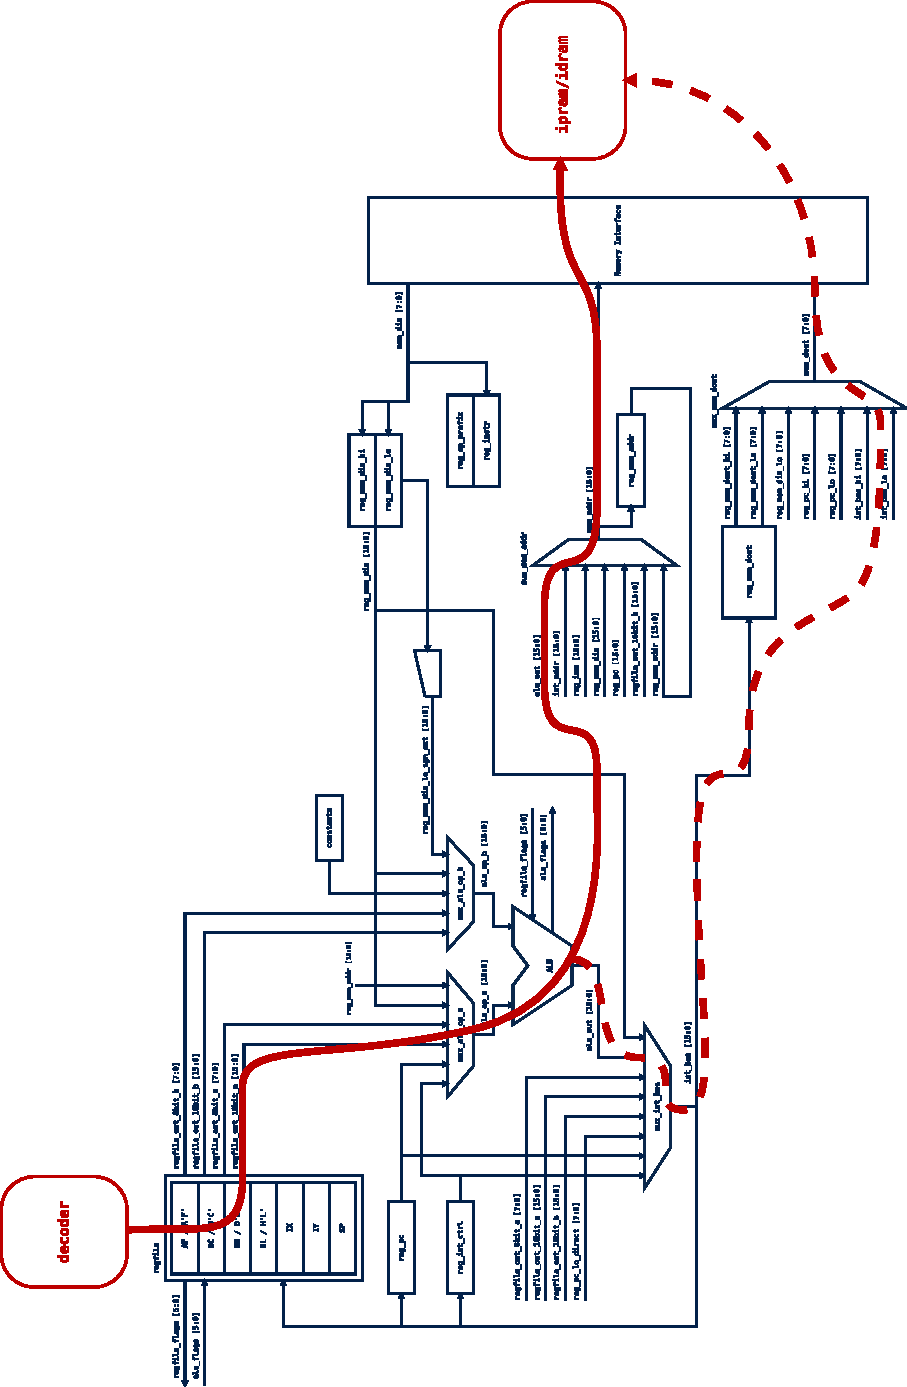
\includegraphics[height=.95\textwidth,angle=-90]{resources/pdf/datapath-critical.pdf}
  \caption{Initialer Kritischer Pfad}
  \label{img:init-critical-path}
\end{figure}

\noindent
Dieser führt vom Decoder über die ALU und den Speicheradressen-Multiplexer zu
einem der internen Speicher\footnote{Teils der interne Programmspeicher, teils
auch der interne Datenspeicher, je nach Synthese-Lauf.}. Dieser Pfad wird unter
anderem von Instruktionen, welche indizierte Adressierung nutzen, benötigt.
Während dieser wird der eingelesene Offset im gleichen Takt, in dem er verfügbar
wird, zu einem der Register \texttt{IX} bzw. \texttt{IY} addiert und das
Ergebnis direkt an die Speicherverwaltung übergeben. Diese entscheidet dann, ob
der Chip-Enable Eingang des internen Datenspeichers aktiviert werden muss. Bei
relativen Sprüngen wird der analoge Pfad zum Programmspeicher genutzt.

Der gestrichelte Pfad führt ebenfalls über die ALU zum internen Datenspeicher.
Über diesen kann das obere oder untere Byte eines ALU-Ergebnisses im gleichen
Takt, in dem es berechnet wird, an den Datenausgang \texttt{mem\_dout} angelegt
werden. In den Synthese-Läufen war der für diesen Pfad ermittelte Slack stets
sehr nah an dem des kritischen Pfades. Dies legt nahe, dass auch dieser Pfad
einer wesentlichen Erhöhung der Taktfrequenz im Wege steht.

Um diese beiden Pfade aufzubrechen wurden die in
Abbildung~\ref{img:datapath-optimized} gezeigten Änderungen am Datenpfad
vorgenommen.

\begin{figure}[htbp]
  \centering
    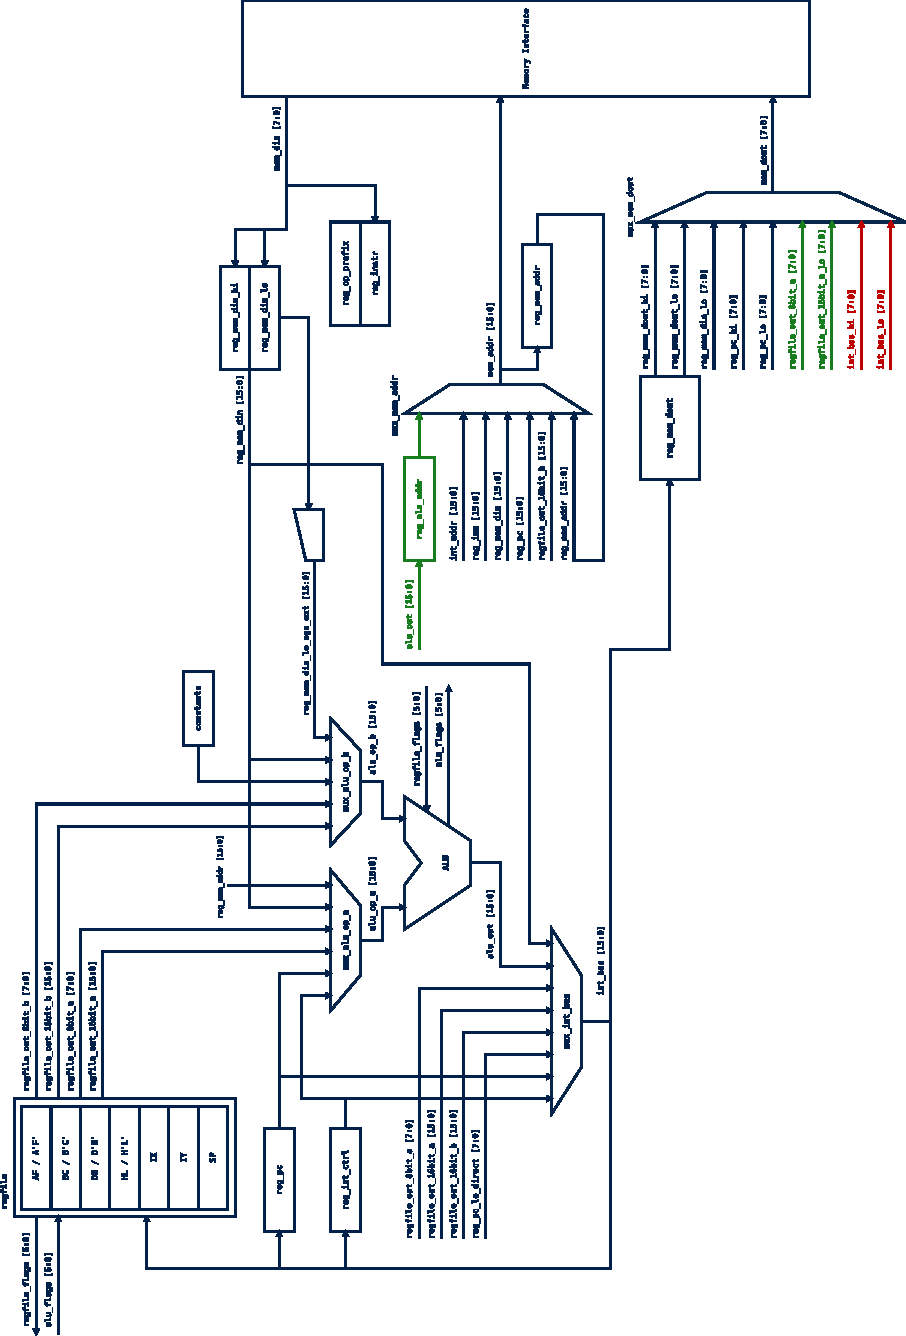
\includegraphics[height=\textwidth,angle=-90]{resources/pdf/datapath-optimized.pdf}
  \caption{Optimierter Datenpfad}
  \label{img:datapath-optimized}
\end{figure}

\noindent
Dabei wurde das zusätzliches Register \texttt{reg\_alu\_addr} zwischen dem
Ausgang der ALU und dem Speicheradressen-Multiplexer eingefügt und der direkte
Pfad über die ALU zum \texttt{mem\_dout} Bus entfernt. Der interne Datenbus
liegt jetzt nur noch über das \texttt{reg\_mem\_dout} Register am
\texttt{mux\_mem\_dout} Multiplexer an, dafür wurden neue direkte Verbindungen
vom Register-File zu diesem hinzugefügt, um Register-Inhalte weiterhin
unverzögert auf den \texttt{mem\_dout} Bus ausgeben zu können.
Da berechnete Adressen und zu schreibende Bytes mit diesen Änderungen nicht
mehr ohne Verzögerung am \texttt{mem\_addr} bzw. \texttt{mem\_dout} Bus
angelegt werden können, musste für von dieser Änderung betroffene Instruktionen
jeweils ein ``Puffer-Takt'' zwischen die die ALU-Operation ausführenden Takte
und die folgenden, auf Speicher oder externe Geräte zugreifenden,
Maschinen-Zyklen eingefügt werden.
Diese Lösung wurde bewusst mit dem Ziel gewählt, die notwendigen Änderungen am
bestehenden Verilog-Code so gering wie möglich zu halten, nur so konnten
die nötigen Anpassungen an Decoder und FSM zeitlich bewältigt werden.

Die den Puffer-Takten entsprechenden Zustände sind in dem in
Abbildung~\ref{img:fsm-states-optimized} dargestellten aktualisierten
Zustandübergangsgraphen gezeigt, der Übersichtlichkeit halber sind nur neu
hinzukommende Zustandsübergänge von und zu den neuen Zuständen gezeigt.

\begin{figure}[htbp]
  \centering
    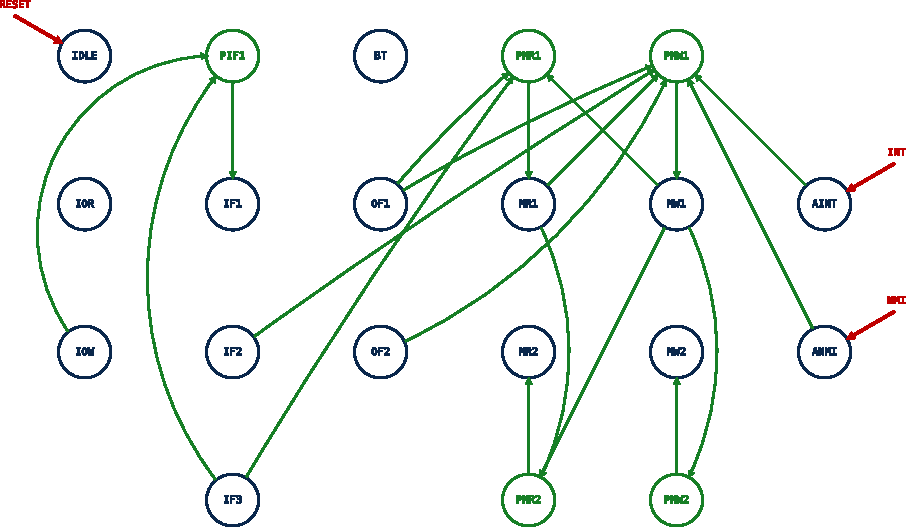
\includegraphics[width=\textwidth]{resources/pdf/fsm-states-optimized.pdf}
  \caption{Zustandsübergänge der Puffer-Zustände}
  \label{img:fsm-states-optimized}
\end{figure}

\begin{figure}[htbp]
  \centering
    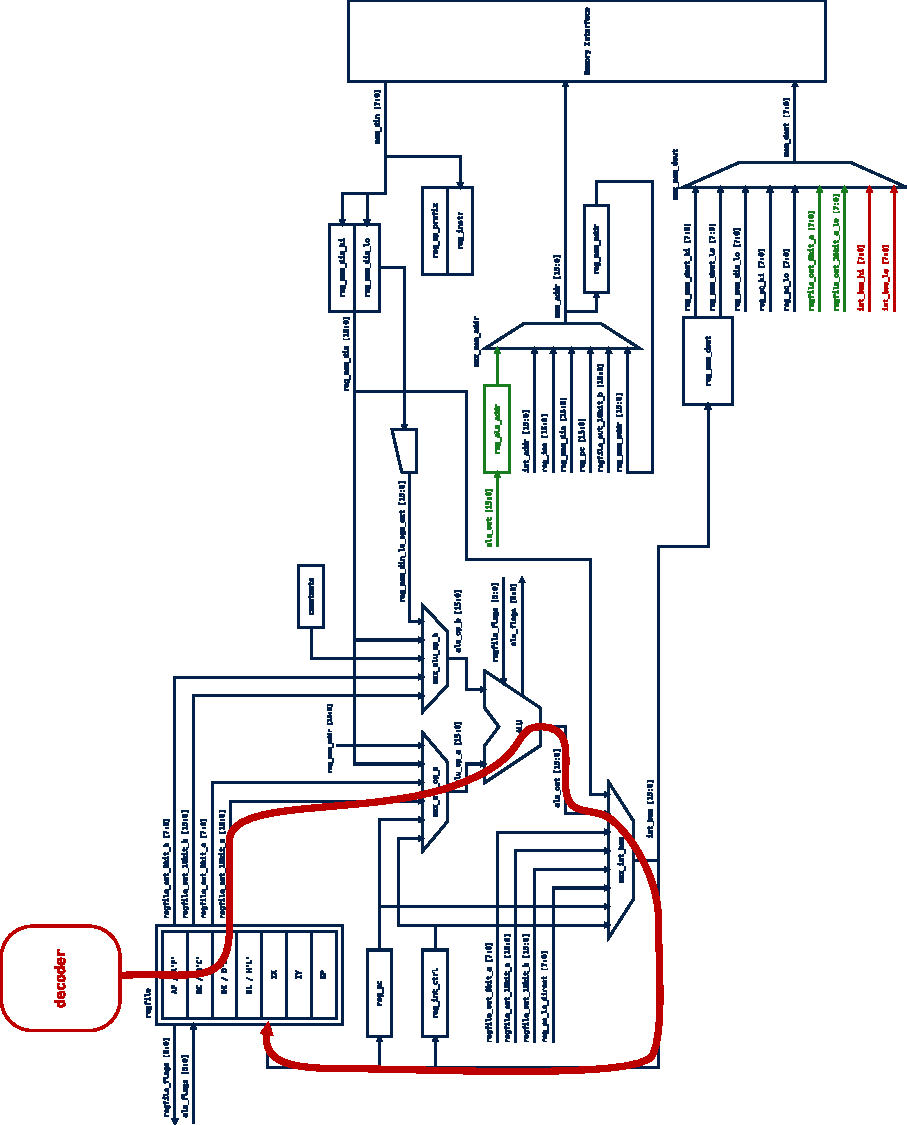
\includegraphics[height=\textwidth,angle=-90]{resources/pdf/datapath-optimized-critical.pdf}
  \caption{Neuer Kritischer Pfad}
  \label{img:datapath-optimized-critical-path}
\end{figure}

Nach erneuter Synthese konnte die Taktrate so bis auf rund 165MHz erhöht
werden. Der neue kritische Pfad ist als Auszug aus dem Timing-Report der
Synthese in Listing~\ref{lst:optimized-critical-path} und grafisch in
Abbildung~\ref{img:datapath-optimized-critical-path} gezeigt und verläuft über
die ALU zum Schreib-Eingang des Register-Files. Ein weiteres Aufbrechen dieses
Pfades ist nicht praktikabel, da das Einfügen von Registern direkt vor oder
hinter der ALU starke Eingriffe in fast allen implementierten Instruktionen
notwendig machen und die durchschnittliche Anzahl von Takten pro Instruktion
deutlich erhöhen würde. Eine weitere Steigerung der Taktfrequenz wäre somit nur
unter erheblicher Neustrukturierung des gesamten Designs denkbar, z.B. durch
Ersetzen der 16-Bit ALU durch eine 8-Bit ALU oder die Einführung einer
Pipeline. Dies war im Rahmen dieses Beleges nicht mehr umsetzbar.

\vskip\baselineskip

\begin{center}
  \begin{minipage}{.8\textwidth}
    \captionof{listing}{Optimierter kritischer Pfad (Auszug \texttt{top\_z80.report\_timing})
    \label{lst:optimized-critical-path}}
    \begin{minted}[frame=none]{text}
Point                                                           Incr       Path
----------------------------------------------------------------------------------
clock CLK (rise edge)                                           0.00       0.00
clock network delay (ideal)                                     1.50       1.50
...
z80_i/cpu_i/datapath_i/reg_instr[7] (datapath)                  0.00       2.04 f
z80_i/cpu_i/controller_i/reg_instr[7] (controller)              0.00       2.04 f
z80_i/cpu_i/controller_i/decoder_i/reg_instr[7] (decoder)
...
z80_i/cpu_i/controller_i/decoder_i/alu_mode[10] (decoder)
                                                                0.00       3.77 f
z80_i/cpu_i/controller_i/alu_mode[10] (controller)              0.00       3.77 f
z80_i/cpu_i/datapath_i/alu_mode[10] (datapath)                  0.00       3.77 f
z80_i/cpu_i/datapath_i/alu_i/mode[10] (alu)                     0.00       3.77 f
...
z80_i/cpu_i/datapath_i/alu_i/data_out[9] (alu)                  0.00       6.63 r
z80_i/cpu_i/datapath_i/mux_int_bus_i/alu_out[9] (mux_int_bus)
                                                                0.00       6.63 r
...
z80_i/cpu_i/datapath_i/mux_int_bus_i/data_out[9] (mux_int_bus)
                                                                0.00       6.91 r
z80_i/cpu_i/datapath_i/regfile_i/reg_in[9] (regfile)
...
data arrival time                                                          7.19

clock CLK (rise edge)                                           6.05       6.05
clock network delay (ideal)                                     1.50       7.55
clock uncertainty                                              -0.20       7.35
...
library setup time                                             -0.16       7.19
data required time                                                         7.19
----------------------------------------------------------------------------------
data required time                                                         7.19
data arrival time                                                         -7.19
----------------------------------------------------------------------------------
slack (MET)                                                                0.00
    \end{minted}
  \end{minipage}
\end{center}

\vskip\baselineskip

\noindent
Ob die erreichte Steigerung der Taktfrequenz von rund 10\% das Einfügen der
Puffer-Takte wert ist, ist nicht eindeutig zu beantworten. Die Ausführungszeit
der meisten betroffenen Instruktionen wird hierdurch verlängert, andererseits
ist die Struktur vieler Instruktionen überhaupt nicht von der Änderung
betroffen, diese profitieren daher von der höheren Taktfrequenz. Intuitiv
überwiegt dieser Vorteil, da beispielsweise arithmetische und logische
Operationen mit indizierter Adressierung in einer typischen Anwendung mit
deutlich geringerer Häufigkeit auftreten als solche, die nicht auf den Speicher
zugreifen oder diesen direkt adressieren. Die erläuterten Optimierungen wurden
daher in die finale Implementierung übernommen.

\chapter{Place \& Route}

Abbildung~\ref{img:post-route} zeigt das Ergebnis des Place \& Route Schrittes.
Der Chip hat eine Gesamtfläche von $1750 x 1012 \mu m^2$ und eine
Gatter-Platzierungsdichte von $66.117\%$. Die Platzierung der Speicherelemente
wurde mit Hinblick darauf gewählt, einfaches Routing von den Anschlüssen ins
Innere des Chips und zu den IO-Pins zu ermöglichen.

\begin{figure}[htbp]
  \centering
    
\includegraphics[width=0.69\textwidth]{resources/png/post-route.png}
  \caption{Place \& Route Ergebnis}
  \label{img:post-route}
\end{figure}

\noindent
Die in Listing~\ref{lst:post-route-summary} gezeigte Post-Route Zusammenfassung
zeigt, dass durch den Place \& Route Schritt keine Timing-Verletzungen
entstanden sind.

\begin{center}
  \begin{minipage}{0.65\textwidth}
    \captionof{listing}{Post-Route Ergebnis (Ausschnitt)\label{lst:post-route-summary}}
    \begin{minted}[frame=none]{text}
---------------------------------------------------------------------
     optDesign Final SI Timing Summary
---------------------------------------------------------------------

+--------------------+---------+---------+---------+---------+
|     Setup mode     |   all   | reg2reg |reg2cgate| default |
+--------------------+---------+---------+---------+---------+
|           WNS (ns):|  0.330  |  0.425  |  0.743  |  0.330  |
|           TNS (ns):|  0.000  |  0.000  |  0.000  |  0.000  |
|    Violating Paths:|    0    |    0    |    0    |    0    |
|          All Paths:|   893   |   429   |   24    |   466   |
+--------------------+---------+---------+---------+---------+

+----------------+-------------------------------+------------------+
|                |              Real             |       Total      |
|    DRVs        +------------------+------------+------------------|
|                |  Nr nets(terms)  | Worst Vio  |  Nr nets(terms)  |
+----------------+------------------+------------+------------------+
|   max_cap      |      0 (0)       |   0.000    |      0 (0)       |
|   max_tran     |      0 (0)       |   0.000    |      0 (0)       |
|   max_fanout   |      0 (0)       |     0      |      0 (0)       |
|   max_length   |      0 (0)       |     0      |      0 (0)       |
+----------------+------------------+------------+------------------+

Density: 66.117%
Total number of glitch violations: 0
---------------------------------------------------------------------
    \end{minted}
  \end{minipage}
\end{center}

\chapter{Abschließende Bewertung}

Insgesamt ist das erzielte Ergebnis absolut zufriendstellend, als Haupterfolg
sehen wir die ausführliche Verifizierung, die uns großes Vertrauen in die
Korrektheit unserer Implementierung gibt. Wenn man das Verhältnis der für die
vereinzelten manuell und die automatisiert erzeugten Testfälle benötigten
Enwicklungsdauer betrachtet, ist zudem davon auszugehen, dass \texttt{ictest}
trotz anfangs hohem Entwicklungswand insgesamt zu einer enormen Zeitersparnis
geführt hat, ohne die im gegebenen Zeitrahmen eine angemessene Verifizierung
unmöglich gewesen wäre.

Bei der eigentlichen Implementierung ist der von uns anfangs angedachte Plan
zur Verfolgung unseres Design-Ziels aufgegangen. Es konnte eine angemessen hohe
Taktfrequenz erzielt werden, bei gleichzeitiger (im Schnitt) niedriger Anzahl
von Takten pro Instruktion. Es wäre jedoch unter Umständen sinnvoll gewesen,
die Optimierung nicht erst am Ende des Entwicklungsprozesses vorzunehmen,
sondern gleich zu Beginn mit verschiedenen möglichen Datenpfaden und deren
kritischen Pfaden in Isolation zu experimentieren. Mit dem von uns verfolgten
Ansatz konnten während der Optimierung nur noch moderate Änderungen am
Datenpfad vorgenommen werden.  Ob fundamental verschiedene Datenpfad-Layouts zu
besseren Ergebnissen geführt hätten bleibt unklar. Es war uns jedoch zu Anfang
noch nicht bewusst, ob dieser zusätzliche Aufwand überhaupt gerechtfertigt
gewesen wäre. Letztlich hätten auch vom Datenpfad-Layout unabhängige Faktoren
die Taktfrequenz limitieren können.

Im Allgemeinen sind Teile des Designs ``organisch'' gewachsen. Es wurden zwar
vor Beginn der Implementierung Schaltpläne für den Datenpfad und grobe
Ablaufpläne für die wichtigsten Instruktionen (d.h. notwendige
Zustandsübergänge) angelegt, diese wurden aber immer wieder angepasst und
erweitert um neuen, durch komplexere Instruktionen bedingten Anforderungen
gerecht zu werden. Es wäre auch denkbar gewesen, mittels einer kompletten
Analyse aller Instruktionen und spezieller Prozessor-Funktionalitäten das
gesamte Design auszuplanen und erst dann mit der Implementierung zu beginnen
(die dann im Idealfall nur noch Formsache gewesen wäre). Wir haben uns aufgrund
unserer mangelnden Erfahrung mit dem Entwurf von CISC Prozessoren gegen diesen
Ansatz entschieden. Mit hoher Wahrscheinlichkeit hätten ohnehin erst während
der Implementierung aufgedeckte Probleme im initialen Design behoben werden
müssen.

\headingsvskip=-120pt

\clearpage
\begingroup
  \let\clearpage\relax
  \phantomsection
  \addcontentsline{toc}{chapter}{\listfigurename}
  \listoffigures
  \phantomsection
  \addcontentsline{toc}{chapter}{Listingverzeichnis}
  \listof{listing}{Listingverzeichnis}
\endgroup

\end{document}
